\chapter{\emph{lemon-tree}: Representing Topical Thesauri on the Semantic Web}
\chaptermark{\emph{lemon-tree}}

%\titlerunning{\emph{lemon-tree}}

%\author{Sander Stolk}{Leiden University, Leiden, The Netherlands}{s.s.stolk@hum.leidenuniv.nl}{https://orcid.org/0000-0003-2254-6613}{}
%\authorrunning{S. Stolk}
%\Copyright{Sander Stolk}

%\keywords{lemon-tree, lemon, OntoLex, SKOS, thesaurus, topical thesaurus, onomasiological ordering, linked data}

% specific to ACM DL publications
%\begin{CCSXML}
%	<ccs2012>
%	<concept>
%	<concept_id>10002951.10003260.10003309.10003315</concept_id>
%	<concept_desc>Information systems~Semantic web description languages</concept_desc>
%	<concept_significance>500</concept_significance>
%	</concept>
%	<concept>
%	<concept_id>10002951.10003317.10003318.10011149</concept_id>
%	<concept_desc>Information systems~Thesauri</concept_desc>
%	<concept_significance>500</concept_significance>
%	</concept>
%	</ccs2012>
%\end{CCSXML}
%\ccsdesc[500]{Information systems~Semantic web description languages}
%\ccsdesc[500]{Information systems~Thesauri}

%\maketitle  % typeset the title of the contribution

\begin{abstract}
An increasing number of dictionaries are represented on the Web in the form of linguistic linked data using the \emph{lemon} vocabulary. Such a representation facilitates interoperability across linguistic resources, has the potential to increase their visibility, and promotes their reuse. Lexicographic resources other than dictionaries have thus far not been the main focus of efforts surrounding \emph{lemon} and its modules. In this paper, fundamental needs are analysed for representing topical thesauri specifically and a solution is provided for two important areas hitherto problematic: (1) levels that can be distinguished in their topical system and (2) a looser form of categorization than lexicalization. The novel \emph{lemon-tree} model contains terminology to overcome these issues and acts as bridge between existing Web standards in order to bring topical thesauri, too, to the Semantic Web.
\end{abstract}

%%%%%%%%%%%%%%%%%%%%%%%%%%%%%%%%%%%%%%%%%%%%%%%%%%%%%%%%%%%%%%%%%%%%%%

\section{Introduction}

An increasing number of dictionaries are represented on the Web in the form of linguistic linked data using the \emph{lemon} vocabulary (e.g. \cite{citeulike:14024090, DBLP:conf/esws/KhanDM16}). Such a representation facilitates interoperability across linguistic resources, has the potential to increase their visibility, and promotes their reuse \cite{declerck-2015, klimek2015enhancing}. The core of the \emph{lemon} vocabulary, OntoLex, has been designed to capture lexicons and to add their lexicographical knowledge to ontologies on the Web \cite{ref-LEMON}. As capturing lexicographic information was not part of the primary aim of OntoLex, recent modules for \emph{lemon} have sought to improve support for expressing such information \cite{DBLP:conf/esws/KhanDM16, citeulike:14396375}. Using these modules, content of lexicographic resources can become part of the Linguistic Linked Data Cloud whilst minimizing information loss in the transition \cite{citeulike:14396375}. These modules, however, have explored mainly the need to represent dictionaries but not other lexicographical works such as topical thesauri. Indeed, previous research points out that additional terminology is needed for such thesauri \cite{stolk-2017}. The current paper aims to fill this gap by putting forward a novel model for this purpose: \emph{lemon-tree}. 

A topical thesaurus is a lexicographical work that organizes its lexical items according to their meaning (rather than alphabetically) by means of a topical structure \cite{brown_thesauruses_2006, kay_diachronic_2016}.
This overarching structure offers generic meanings to users as a starting point, which branch out to meanings increasingly specific. Once users locate the meaning which they are interested in, they are presented with the words or phrases that express that meaning. This overarching topical system in a thesaurus thus allows the user to move from meaning to lexical item \cite{hullen_history_2004}.

The new \emph{lemon-tree} vocabulary, described in this paper, bridges the existing standards SKOS \cite{ref-SKOS} and \emph{lemon} in order to express the content of topical thesauri on the Web. The SKOS vocabulary already allows for sharing concepts in RDF and organizing them in hierarchies. The \emph{lemon} model and its core module OntoLex allow for sharing lexical entries, senses, and further lexicographic material. Terminology from both the SKOS and \emph{lemon} standards, then, are valuable for sharing topical thesauri on the Web in an interoperable manner. The \emph{lemon-tree} model therefore aims to facilitate their combined use for that purpose, adding some terminology for perceived lacunae.


\section{Methodology}

In order to provide insight into fundamental needs for representing topical thesauri on the Web beyond those for other lexicographic material (e.g., dictionaries), this paper will explore elements specific to the structure of topical thesauri. For each such element or structuring, the extent is discussed with which SKOS and \emph{lemon} OntoLex offer terminology to represent these elements. For lacunae, available terminology in the new \emph{lemon-tree} model is discussed that is fit for the purpose. Each topic is illustrated by means of an existing thesaurus that exemplifies the matter at hand. Listed in order of their appearance, these thesauri are:

\begin{itemize}
	\item Historical Thesaurus of the Oxford English Dictionary (HTOED) \cite{ref-HTOED}
	\item Shakespeare Thesaurus (ShT) \cite{ref-ShT}
	\item Scots Thesaurus (ScT) \cite{ref-ScT}
	\item Love, Sex, and Marriage (LSM) \cite{ref-LSM}
	\item Roget's Thesaurus (Roget's) \cite{ref-Roget}
\end{itemize}

\noindent
Figure \ref{fig:Stolk2019a:legend} is a legend to the images in this paper that depict the content of existing thesauri.

\begin{figure}[htbp]
	\framebox[\textwidth]{
		\scalebox{0.7}[0.7]{
			% Graphic for TeX using PGF
% Title: C:\Users\Sander\Documents\Dropbox\PhD\images\legend.dia
% Creator: Dia v0.97.2
% CreationDate: Wed Jan 02 16:12:26 2019
% For: Sander
% \usepackage{tikz}
% The following commands are not supported in PSTricks at present
% We define them conditionally, so when they are implemented,
% this pgf file will use them.
\ifx\du\undefined
  \newlength{\du}
\fi
\setlength{\du}{15\unitlength}
\begin{tikzpicture}
\pgftransformxscale{1.000000}
\pgftransformyscale{-1.000000}
\definecolor{dialinecolor}{rgb}{0.000000, 0.000000, 0.000000}
\pgfsetstrokecolor{dialinecolor}
\definecolor{dialinecolor}{rgb}{1.000000, 1.000000, 1.000000}
\pgfsetfillcolor{dialinecolor}
\pgfsetlinewidth{0.100000\du}
\pgfsetdash{}{0pt}
\pgfsetdash{}{0pt}
\pgfsetmiterjoin
\pgfsetbuttcap
{
\definecolor{dialinecolor}{rgb}{0.000000, 0.000000, 1.000000}
\pgfsetfillcolor{dialinecolor}
% was here!!!
\pgfsetarrowsend{stealth}
{\pgfsetcornersarced{\pgfpoint{0.000000\du}{0.000000\du}}\definecolor{dialinecolor}{rgb}{0.000000, 0.000000, 1.000000}
\pgfsetstrokecolor{dialinecolor}
\draw (2.050000\du,4.950000\du)--(1.195810\du,4.950000\du)--(1.195810\du,3.100000\du)--(1.195810\du,3.100000\du);
}}
\pgfsetlinewidth{0.100000\du}
\pgfsetdash{}{0pt}
\pgfsetdash{}{0pt}
\pgfsetbuttcap
\pgfsetmiterjoin
\pgfsetlinewidth{0.100000\du}
\pgfsetbuttcap
\pgfsetmiterjoin
\pgfsetdash{}{0pt}
\definecolor{dialinecolor}{rgb}{1.000000, 0.984314, 0.435294}
\pgfsetfillcolor{dialinecolor}
\pgfpathellipse{\pgfpoint{1.190000\du}{1.200000\du}}{\pgfpoint{1.000000\du}{0\du}}{\pgfpoint{0\du}{1.000000\du}}
\pgfusepath{fill}
\definecolor{dialinecolor}{rgb}{0.000000, 0.000000, 0.000000}
\pgfsetstrokecolor{dialinecolor}
\pgfpathellipse{\pgfpoint{1.190000\du}{1.200000\du}}{\pgfpoint{1.000000\du}{0\du}}{\pgfpoint{0\du}{1.000000\du}}
\pgfusepath{stroke}
\pgfsetbuttcap
\pgfsetmiterjoin
\pgfsetdash{}{0pt}
\definecolor{dialinecolor}{rgb}{0.000000, 0.000000, 0.000000}
\pgfsetstrokecolor{dialinecolor}
\pgfpathellipse{\pgfpoint{1.190000\du}{1.200000\du}}{\pgfpoint{1.000000\du}{0\du}}{\pgfpoint{0\du}{1.000000\du}}
\pgfusepath{stroke}
\definecolor{dialinecolor}{rgb}{1.000000, 1.000000, 1.000000}
\pgfsetfillcolor{dialinecolor}
\fill (3.898750\du,0.707500\du)--(3.898750\du,1.695000\du)--(8.493750\du,1.695000\du)--(8.493750\du,0.707500\du)--cycle;
% setfont left to latex
\definecolor{dialinecolor}{rgb}{0.000000, 0.000000, 0.000000}
\pgfsetstrokecolor{dialinecolor}
\node[anchor=west] at (3.898750\du,1.495000\du){A semantic concept / category};
\definecolor{dialinecolor}{rgb}{1.000000, 1.000000, 1.000000}
\pgfsetfillcolor{dialinecolor}
\fill (3.845000\du,3.550000\du)--(3.845000\du,4.537500\du)--(14.302500\du,4.537500\du)--(14.302500\du,3.550000\du)--cycle;
% setfont left to latex
\definecolor{dialinecolor}{rgb}{0.000000, 0.000000, 0.000000}
\pgfsetstrokecolor{dialinecolor}
\node[anchor=west] at (3.845000\du,4.337500\du){Categorization of senses};
\pgfsetlinewidth{0.100000\du}
\pgfsetdash{}{0pt}
\pgfsetdash{}{0pt}
\pgfsetmiterjoin
\definecolor{dialinecolor}{rgb}{1.000000, 1.000000, 1.000000}
\pgfsetfillcolor{dialinecolor}
\fill (17.895000\du,0.300000\du)--(17.895000\du,2.000000\du)--(19.800000\du,2.000000\du)--(19.800000\du,0.300000\du)--cycle;
\definecolor{dialinecolor}{rgb}{0.000000, 0.000000, 1.000000}
\pgfsetstrokecolor{dialinecolor}
\draw (17.895000\du,0.300000\du)--(17.895000\du,2.000000\du)--(19.800000\du,2.000000\du)--(19.800000\du,0.300000\du)--cycle;
\definecolor{dialinecolor}{rgb}{1.000000, 1.000000, 1.000000}
\pgfsetfillcolor{dialinecolor}
\fill (21.245000\du,0.600000\du)--(21.245000\du,1.587500\du)--(27.605000\du,1.587500\du)--(27.605000\du,0.600000\du)--cycle;
% setfont left to latex
\definecolor{dialinecolor}{rgb}{0.000000, 0.000000, 0.000000}
\pgfsetstrokecolor{dialinecolor}
\node[anchor=west] at (21.245000\du,1.387500\du){A list of senses};
\pgfsetlinewidth{0.100000\du}
\pgfsetdash{}{0pt}
\pgfsetdash{}{0pt}
\pgfsetmiterjoin
\definecolor{dialinecolor}{rgb}{1.000000, 1.000000, 1.000000}
\pgfsetfillcolor{dialinecolor}
\fill (17.945000\du,3.250000\du)--(17.945000\du,4.950000\du)--(19.850000\du,4.950000\du)--(19.850000\du,3.250000\du)--cycle;
\definecolor{dialinecolor}{rgb}{0.000000, 0.000000, 1.000000}
\pgfsetstrokecolor{dialinecolor}
\draw (17.945000\du,3.250000\du)--(17.945000\du,4.950000\du)--(19.850000\du,4.950000\du)--(19.850000\du,3.250000\du)--cycle;
\pgfsetlinewidth{0.100000\du}
\pgfsetdash{}{0pt}
\pgfsetdash{}{0pt}
\pgfsetmiterjoin
\definecolor{dialinecolor}{rgb}{0.000000, 0.000000, 1.000000}
\pgfsetfillcolor{dialinecolor}
\fill (17.945000\du,3.250000\du)--(17.945000\du,3.800000\du)--(19.850000\du,3.800000\du)--(19.850000\du,3.250000\du)--cycle;
\definecolor{dialinecolor}{rgb}{0.000000, 0.000000, 1.000000}
\pgfsetstrokecolor{dialinecolor}
\draw (17.945000\du,3.250000\du)--(17.945000\du,3.800000\du)--(19.850000\du,3.800000\du)--(19.850000\du,3.250000\du)--cycle;
\definecolor{dialinecolor}{rgb}{1.000000, 1.000000, 1.000000}
\pgfsetfillcolor{dialinecolor}
\fill (21.245000\du,3.500000\du)--(21.245000\du,4.487500\du)--(33.237500\du,4.487500\du)--(33.237500\du,3.500000\du)--cycle;
% setfont left to latex
\definecolor{dialinecolor}{rgb}{0.000000, 0.000000, 0.000000}
\pgfsetstrokecolor{dialinecolor}
\node[anchor=west] at (21.245000\du,4.287500\du){A list of synonymous senses};
% setfont left to latex
\definecolor{dialinecolor}{rgb}{1.000000, 1.000000, 1.000000}
\pgfsetstrokecolor{dialinecolor}
\node[text=white] at (18.897500\du,3.650000\du){syno.};
\end{tikzpicture}

		}
	}
	\caption[]{\label{fig:Stolk2019a:legend} Legend}
\end{figure} 

Namespaces of the vocabularies relevant for this paper are provided in Listing \ref{lst:Stolk2019a:namespaces}. The RDF snippets in subsequent listings are specified in the Turtle RDF syntax \cite{prudhommeaux_rdf_2014}. In these snippets, samples taken from existing thesauri correspond with resources between angular brackets (that is to say, their namespace is left unspecified for the present purpose).

\noindent
\begin{minipage}[c]{\textwidth}
	\begin{lstlisting}[
	caption={Namespaces},
	label={lst:Stolk2019a:namespaces}
	]
	@prefix tree: <https://w3id.org/lemon-tree#> .
	@prefix ontolex: <http://www.w3.org/ns/lemon/ontolex#> .
	@prefix skos: <http://www.w3.org/2004/02/skos#> .
	@prefix dcterms: <http://purl.org/dc/terms/> .
	@prefix rdf: <http://www.w3.org/1999/02/22-rdf-syntax-ns#> .
	@prefix rdfs: <http://www.w3.org/2000/01/rdf-schema#> .
	@prefix owl: <http://www.w3.org/2002/07/owl#> .
	@prefix xsd: <http://www.w3.org/2001/XMLSchema#> .
	\end{lstlisting}
\end{minipage}

Before going to the analysis proper, the next section will first provide a short background on topical thesauri. The section that follows treats the topical system, along with the different kinds of levels distinguished in such a system. Afterwards, words and their place within the topical system are discussed, followed by the conclusion.



\section{Topical thesaurus}

A topical thesaurus is a lexicographic resource that organizes its items according to their meaning rather than alphabetically \cite{brown_thesauruses_2006} \cite{kay_diachronic_2016}. They do this by means of a topical structure: a tree of concepts. This overarching structure offers generic meanings to users as a starting point, which branch out to meanings increasingly specific. Once users locate the meaning which they are interested in, they are presented with the words or phrases that express that meaning. This overarching topical system in a thesaurus thus allows the user to move from meaning to lexical item. Figure \ref{fig:Stolk2019a:HTE} displays the main components of such a thesaurus, using a sample of the Historical Thesaurus of the Oxford English Dictionary \cite{ref-HTOED}. The senses of four nouns are shown to be categorized under "Freedom/liberty" (of which those marked with a cross no longer exist). As these four senses convey the same meaning, they are thought to be loosely synonymous.

% Dia export had to be mended slightly:
% - font colour was not applied (made 'synonyms' white)
% - bold font effect was not applied (made 'synonyms' bold)
% - dagger symbol did not appear (replaced † with $\dagger$)
% - synonym box had to be expanded (replaced 35.* values to 36.*) 
\begin{figure}[htbp]
	\framebox[\textwidth]{
		\scalebox{0.65}[0.65]{
			% Graphic for TeX using PGF
% Title: C:\Users\Sander\Documents\Dropbox\PhD\images\Content-parts.dia
% Creator: Dia v0.97.2
% CreationDate: Mon Apr 03 08:42:47 2017
% For: Sander
% \usepackage{tikz}
% The following commands are not supported in PSTricks at present
% We define them conditionally, so when they are implemented,
% this pgf file will use them.
\ifx\du\undefined
  \newlength{\du}
\fi
\setlength{\du}{15\unitlength}
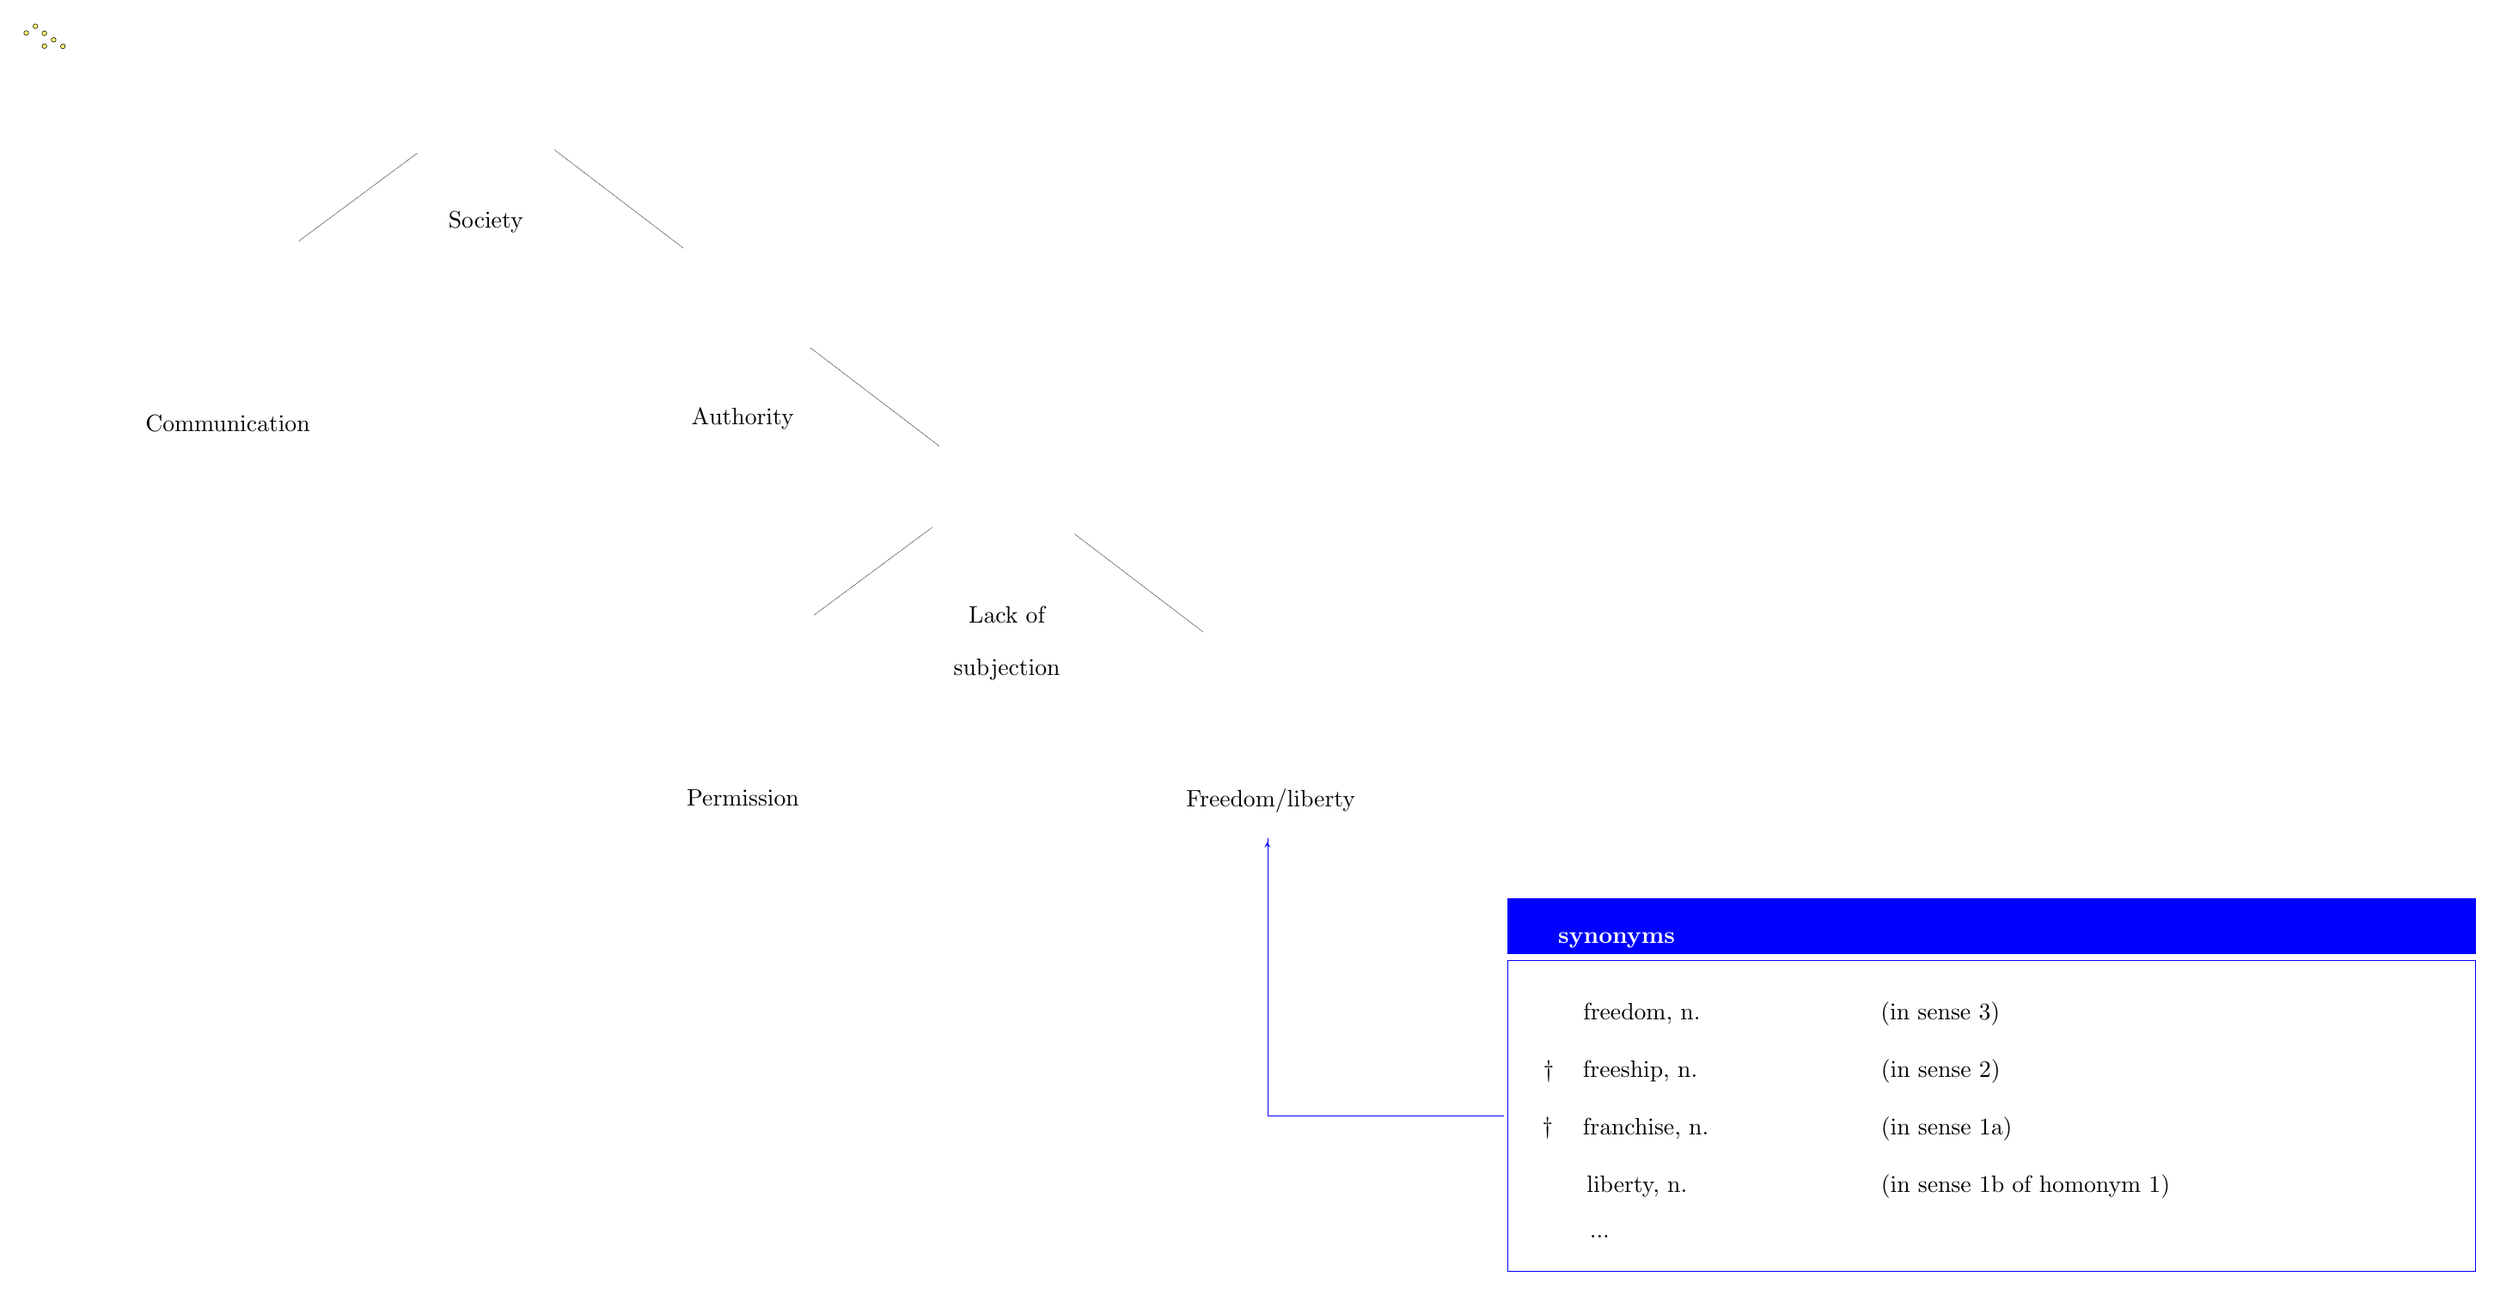
\begin{tikzpicture}
\pgftransformxscale{1.000000}
\pgftransformyscale{-1.000000}
\definecolor{dialinecolor}{rgb}{0.000000, 0.000000, 0.000000}
\pgfsetstrokecolor{dialinecolor}
\definecolor{dialinecolor}{rgb}{1.000000, 1.000000, 1.000000}
\pgfsetfillcolor{dialinecolor}
\pgfsetlinewidth{0.100000\du}
\pgfsetdash{}{0pt}
\pgfsetdash{}{0pt}
\pgfsetbuttcap
\pgfsetmiterjoin
\pgfsetlinewidth{0.100000\du}
\pgfsetbuttcap
\pgfsetmiterjoin
\pgfsetdash{}{0pt}
\definecolor{dialinecolor}{rgb}{1.000000, 0.984314, 0.435294}
\pgfsetfillcolor{dialinecolor}
\pgfpathellipse{\pgfpoint{14.600000\du}{6.900000\du}}{\pgfpoint{1.000000\du}{0\du}}{\pgfpoint{0\du}{1.000000\du}}
\pgfusepath{fill}
\definecolor{dialinecolor}{rgb}{0.000000, 0.000000, 0.000000}
\pgfsetstrokecolor{dialinecolor}
\pgfpathellipse{\pgfpoint{14.600000\du}{6.900000\du}}{\pgfpoint{1.000000\du}{0\du}}{\pgfpoint{0\du}{1.000000\du}}
\pgfusepath{stroke}
\pgfsetbuttcap
\pgfsetmiterjoin
\pgfsetdash{}{0pt}
\definecolor{dialinecolor}{rgb}{0.000000, 0.000000, 0.000000}
\pgfsetstrokecolor{dialinecolor}
\pgfpathellipse{\pgfpoint{14.600000\du}{6.900000\du}}{\pgfpoint{1.000000\du}{0\du}}{\pgfpoint{0\du}{1.000000\du}}
\pgfusepath{stroke}
\pgfsetlinewidth{0.100000\du}
\pgfsetdash{}{0pt}
\pgfsetdash{}{0pt}
\pgfsetmiterjoin
\definecolor{dialinecolor}{rgb}{1.000000, 1.000000, 1.000000}
\pgfsetfillcolor{dialinecolor}
\fill (22.000000\du,13.850000\du)--(22.000000\du,18.450000\du)--(36.300000\du,18.450000\du)--(36.300000\du,13.850000\du)--cycle;
\definecolor{dialinecolor}{rgb}{0.000000, 0.000000, 1.000000}
\pgfsetstrokecolor{dialinecolor}
\draw (22.000000\du,13.850000\du)--(22.000000\du,18.450000\du)--(36.300000\du,18.450000\du)--(36.300000\du,13.850000\du)--cycle;
% setfont left to latex
\definecolor{dialinecolor}{rgb}{0.000000, 0.000000, 0.000000}
\pgfsetstrokecolor{dialinecolor}
\node[anchor=west] at (23.050000\du,17.200000\du){liberty, n.};
% setfont left to latex
\definecolor{dialinecolor}{rgb}{0.000000, 0.000000, 0.000000}
\pgfsetstrokecolor{dialinecolor}
\node[anchor=west] at (23.000000\du,14.650000\du){freedom, n.};
\pgfsetlinewidth{0.100000\du}
\pgfsetdash{}{0pt}
\pgfsetdash{}{0pt}
\pgfsetmiterjoin
\pgfsetbuttcap
{
\definecolor{dialinecolor}{rgb}{0.000000, 0.000000, 1.000000}
\pgfsetfillcolor{dialinecolor}
% was here!!!
\pgfsetarrowsend{stealth}
{\pgfsetcornersarced{\pgfpoint{0.000000\du}{0.000000\du}}\definecolor{dialinecolor}{rgb}{0.000000, 0.000000, 1.000000}
\pgfsetstrokecolor{dialinecolor}
\draw (21.949713\du,16.150000\du)--(18.450000\du,16.150000\du)--(18.450000\du,12.100000\du)--(18.450000\du,12.100000\du);
}}
\definecolor{dialinecolor}{rgb}{1.000000, 1.000000, 1.000000}
\pgfsetfillcolor{dialinecolor}
\fill (16.050000\du,13.805000\du)--(16.050000\du,14.550000\du)--(16.050000\du,14.550000\du)--(16.050000\du,13.805000\du)--cycle;
% setfont left to latex
\definecolor{dialinecolor}{rgb}{0.000000, 0.000000, 0.000000}
\pgfsetstrokecolor{dialinecolor}
\node at (16.050000\du,14.400000\du){};
\definecolor{dialinecolor}{rgb}{1.000000, 1.000000, 1.000000}
\pgfsetfillcolor{dialinecolor}
\fill (12.726250\du,8.155000\du)--(12.726250\du,9.700000\du)--(16.473750\du,9.700000\du)--(16.473750\du,8.155000\du)--cycle;
% setfont left to latex
\definecolor{dialinecolor}{rgb}{0.000000, 0.000000, 0.000000}
\pgfsetstrokecolor{dialinecolor}
\node at (14.600000\du,8.750000\du){Lack of };
% setfont left to latex
\definecolor{dialinecolor}{rgb}{0.000000, 0.000000, 0.000000}
\pgfsetstrokecolor{dialinecolor}
\node at (14.600000\du,9.550000\du){subjection};
\pgfsetlinewidth{0.100000\du}
\pgfsetdash{}{0pt}
\pgfsetdash{}{0pt}
\pgfsetbuttcap
\pgfsetmiterjoin
\pgfsetlinewidth{0.100000\du}
\pgfsetbuttcap
\pgfsetmiterjoin
\pgfsetdash{}{0pt}
\definecolor{dialinecolor}{rgb}{1.000000, 0.984314, 0.435294}
\pgfsetfillcolor{dialinecolor}
\pgfpathellipse{\pgfpoint{10.695000\du}{4.150000\du}}{\pgfpoint{1.000000\du}{0\du}}{\pgfpoint{0\du}{1.000000\du}}
\pgfusepath{fill}
\definecolor{dialinecolor}{rgb}{0.000000, 0.000000, 0.000000}
\pgfsetstrokecolor{dialinecolor}
\pgfpathellipse{\pgfpoint{10.695000\du}{4.150000\du}}{\pgfpoint{1.000000\du}{0\du}}{\pgfpoint{0\du}{1.000000\du}}
\pgfusepath{stroke}
\pgfsetbuttcap
\pgfsetmiterjoin
\pgfsetdash{}{0pt}
\definecolor{dialinecolor}{rgb}{0.000000, 0.000000, 0.000000}
\pgfsetstrokecolor{dialinecolor}
\pgfpathellipse{\pgfpoint{10.695000\du}{4.150000\du}}{\pgfpoint{1.000000\du}{0\du}}{\pgfpoint{0\du}{1.000000\du}}
\pgfusepath{stroke}
\pgfsetlinewidth{0.100000\du}
\pgfsetdash{}{0pt}
\pgfsetdash{}{0pt}
\pgfsetbuttcap
\pgfsetmiterjoin
\pgfsetlinewidth{0.100000\du}
\pgfsetbuttcap
\pgfsetmiterjoin
\pgfsetdash{}{0pt}
\definecolor{dialinecolor}{rgb}{1.000000, 0.984314, 0.435294}
\pgfsetfillcolor{dialinecolor}
\pgfpathellipse{\pgfpoint{6.940000\du}{1.200000\du}}{\pgfpoint{1.000000\du}{0\du}}{\pgfpoint{0\du}{1.000000\du}}
\pgfusepath{fill}
\definecolor{dialinecolor}{rgb}{0.000000, 0.000000, 0.000000}
\pgfsetstrokecolor{dialinecolor}
\pgfpathellipse{\pgfpoint{6.940000\du}{1.200000\du}}{\pgfpoint{1.000000\du}{0\du}}{\pgfpoint{0\du}{1.000000\du}}
\pgfusepath{stroke}
\pgfsetbuttcap
\pgfsetmiterjoin
\pgfsetdash{}{0pt}
\definecolor{dialinecolor}{rgb}{0.000000, 0.000000, 0.000000}
\pgfsetstrokecolor{dialinecolor}
\pgfpathellipse{\pgfpoint{6.940000\du}{1.200000\du}}{\pgfpoint{1.000000\du}{0\du}}{\pgfpoint{0\du}{1.000000\du}}
\pgfusepath{stroke}
\definecolor{dialinecolor}{rgb}{1.000000, 1.000000, 1.000000}
\pgfsetfillcolor{dialinecolor}
\fill (8.991250\du,5.250000\du)--(8.991250\du,5.995000\du)--(12.398750\du,5.995000\du)--(12.398750\du,5.250000\du)--cycle;
% setfont left to latex
\definecolor{dialinecolor}{rgb}{0.000000, 0.000000, 0.000000}
\pgfsetstrokecolor{dialinecolor}
\node at (10.695000\du,5.845000\du){Authority};
\definecolor{dialinecolor}{rgb}{1.000000, 1.000000, 1.000000}
\pgfsetfillcolor{dialinecolor}
\fill (5.570000\du,2.350000\du)--(5.570000\du,3.095000\du)--(8.227500\du,3.095000\du)--(8.227500\du,2.350000\du)--cycle;
% setfont left to latex
\definecolor{dialinecolor}{rgb}{0.000000, 0.000000, 0.000000}
\pgfsetstrokecolor{dialinecolor}
\node at (6.898750\du,2.945000\du){Society};
\pgfsetlinewidth{0.100000\du}
\pgfsetdash{}{0pt}
\pgfsetdash{}{0pt}
\pgfsetbuttcap
{
\definecolor{dialinecolor}{rgb}{0.000000, 0.000000, 0.000000}
\pgfsetfillcolor{dialinecolor}
% was here!!!
\definecolor{dialinecolor}{rgb}{0.000000, 0.000000, 0.000000}
\pgfsetstrokecolor{dialinecolor}
\draw (13.600000\du,6.250000\du)--(11.700000\du,4.800000\du);
}
\pgfsetlinewidth{0.100000\du}
\pgfsetdash{}{0pt}
\pgfsetdash{}{0pt}
\pgfsetbuttcap
{
\definecolor{dialinecolor}{rgb}{0.000000, 0.000000, 0.000000}
\pgfsetfillcolor{dialinecolor}
% was here!!!
\definecolor{dialinecolor}{rgb}{0.000000, 0.000000, 0.000000}
\pgfsetstrokecolor{dialinecolor}
\draw (9.815080\du,3.320080\du)--(7.915080\du,1.870080\du);
}
\pgfsetlinewidth{0.100000\du}
\pgfsetdash{}{0pt}
\pgfsetdash{}{0pt}
\pgfsetmiterjoin
\definecolor{dialinecolor}{rgb}{0.000000, 0.000000, 1.000000}
\pgfsetfillcolor{dialinecolor}
\fill (21.997400\du,12.943200\du)--(21.997400\du,13.755370\du)--(36.300100\du,13.755370\du)--(36.300100\du,12.943200\du)--cycle;
\definecolor{dialinecolor}{rgb}{0.000000, 0.000000, 1.000000}
\pgfsetstrokecolor{dialinecolor}
\draw (21.997400\du,12.943200\du)--(21.997400\du,13.755370\du)--(36.300100\du,13.755370\du)--(36.300100\du,12.943200\du)--cycle;
% setfont left to latex
\definecolor{dialinecolor}{rgb}{1.000000, 1.000000, 1.000000}
\pgfsetstrokecolor{dialinecolor}
\node[anchor=west,white] at (22.629800\du,13.562800\du){\textbf{\textcolor{white}{synonyms}}};
\pgfsetlinewidth{0.100000\du}
\pgfsetdash{}{0pt}
\pgfsetdash{}{0pt}
\pgfsetbuttcap
\pgfsetmiterjoin
\pgfsetlinewidth{0.100000\du}
\pgfsetbuttcap
\pgfsetmiterjoin
\pgfsetdash{}{0pt}
\definecolor{dialinecolor}{rgb}{1.000000, 0.984314, 0.435294}
\pgfsetfillcolor{dialinecolor}
\pgfpathellipse{\pgfpoint{18.500000\du}{9.650000\du}}{\pgfpoint{1.000000\du}{0\du}}{\pgfpoint{0\du}{1.000000\du}}
\pgfusepath{fill}
\definecolor{dialinecolor}{rgb}{0.000000, 0.000000, 0.000000}
\pgfsetstrokecolor{dialinecolor}
\pgfpathellipse{\pgfpoint{18.500000\du}{9.650000\du}}{\pgfpoint{1.000000\du}{0\du}}{\pgfpoint{0\du}{1.000000\du}}
\pgfusepath{stroke}
\pgfsetbuttcap
\pgfsetmiterjoin
\pgfsetdash{}{0pt}
\definecolor{dialinecolor}{rgb}{0.000000, 0.000000, 0.000000}
\pgfsetstrokecolor{dialinecolor}
\pgfpathellipse{\pgfpoint{18.500000\du}{9.650000\du}}{\pgfpoint{1.000000\du}{0\du}}{\pgfpoint{0\du}{1.000000\du}}
\pgfusepath{stroke}
\definecolor{dialinecolor}{rgb}{1.000000, 1.000000, 1.000000}
\pgfsetfillcolor{dialinecolor}
\fill (15.603750\du,10.905000\du)--(15.603750\du,11.650000\du)--(21.396250\du,11.650000\du)--(21.396250\du,10.905000\du)--cycle;
% setfont left to latex
\definecolor{dialinecolor}{rgb}{0.000000, 0.000000, 0.000000}
\pgfsetstrokecolor{dialinecolor}
\node at (18.500000\du,11.500000\du){Freedom/liberty};
\pgfsetlinewidth{0.100000\du}
\pgfsetdash{}{0pt}
\pgfsetdash{}{0pt}
\pgfsetbuttcap
{
\definecolor{dialinecolor}{rgb}{0.000000, 0.000000, 0.000000}
\pgfsetfillcolor{dialinecolor}
% was here!!!
\definecolor{dialinecolor}{rgb}{0.000000, 0.000000, 0.000000}
\pgfsetstrokecolor{dialinecolor}
\draw (17.500000\du,9.000000\du)--(15.600000\du,7.550000\du);
}
% setfont left to latex
\definecolor{dialinecolor}{rgb}{0.000000, 0.000000, 0.000000}
\pgfsetstrokecolor{dialinecolor}
\node[anchor=west] at (22.995000\du,15.495000\du){freeship, n.};
% setfont left to latex
\definecolor{dialinecolor}{rgb}{0.000000, 0.000000, 0.000000}
\pgfsetstrokecolor{dialinecolor}
\node[anchor=west] at (22.995000\du,16.345000\du){franchise, n.};
% setfont left to latex
\definecolor{dialinecolor}{rgb}{0.000000, 0.000000, 0.000000}
\pgfsetstrokecolor{dialinecolor}
\node[anchor=west] at (23.095000\du,17.945000\du){...};
% setfont left to latex
\definecolor{dialinecolor}{rgb}{0.000000, 0.000000, 0.000000}
\pgfsetstrokecolor{dialinecolor}
\node[anchor=west] at (27.395000\du,14.645000\du){(in sense 3)};
\pgfsetlinewidth{0.100000\du}
\pgfsetdash{}{0pt}
\pgfsetdash{}{0pt}
\pgfsetbuttcap
{
\definecolor{dialinecolor}{rgb}{0.000000, 0.000000, 0.000000}
\pgfsetfillcolor{dialinecolor}
% was here!!!
\definecolor{dialinecolor}{rgb}{0.000000, 0.000000, 0.000000}
\pgfsetstrokecolor{dialinecolor}
\draw (13.500000\du,7.450000\du)--(11.750000\du,8.750000\du);
}
\pgfsetlinewidth{0.100000\du}
\pgfsetdash{}{0pt}
\pgfsetdash{}{0pt}
\pgfsetbuttcap
\pgfsetmiterjoin
\pgfsetlinewidth{0.100000\du}
\pgfsetbuttcap
\pgfsetmiterjoin
\pgfsetdash{}{0pt}
\definecolor{dialinecolor}{rgb}{1.000000, 0.984314, 0.435294}
\pgfsetfillcolor{dialinecolor}
\pgfpathellipse{\pgfpoint{10.715080\du}{9.570080\du}}{\pgfpoint{1.000000\du}{0\du}}{\pgfpoint{0\du}{1.000000\du}}
\pgfusepath{fill}
\definecolor{dialinecolor}{rgb}{0.000000, 0.000000, 0.000000}
\pgfsetstrokecolor{dialinecolor}
\pgfpathellipse{\pgfpoint{10.715080\du}{9.570080\du}}{\pgfpoint{1.000000\du}{0\du}}{\pgfpoint{0\du}{1.000000\du}}
\pgfusepath{stroke}
\pgfsetbuttcap
\pgfsetmiterjoin
\pgfsetdash{}{0pt}
\definecolor{dialinecolor}{rgb}{0.000000, 0.000000, 0.000000}
\pgfsetstrokecolor{dialinecolor}
\pgfpathellipse{\pgfpoint{10.715080\du}{9.570080\du}}{\pgfpoint{1.000000\du}{0\du}}{\pgfpoint{0\du}{1.000000\du}}
\pgfusepath{stroke}
\definecolor{dialinecolor}{rgb}{1.000000, 1.000000, 1.000000}
\pgfsetfillcolor{dialinecolor}
\fill (8.708750\du,10.855000\du)--(8.708750\du,11.600000\du)--(12.691250\du,11.600000\du)--(12.691250\du,10.855000\du)--cycle;
% setfont left to latex
\definecolor{dialinecolor}{rgb}{0.000000, 0.000000, 0.000000}
\pgfsetstrokecolor{dialinecolor}
\node at (10.700000\du,11.450000\du){Permission};
\pgfsetlinewidth{0.100000\du}
\pgfsetdash{}{0pt}
\pgfsetdash{}{0pt}
\pgfsetbuttcap
{
\definecolor{dialinecolor}{rgb}{0.000000, 0.000000, 0.000000}
\pgfsetfillcolor{dialinecolor}
% was here!!!
\definecolor{dialinecolor}{rgb}{0.000000, 0.000000, 0.000000}
\pgfsetstrokecolor{dialinecolor}
\draw (5.886250\du,1.919950\du)--(4.136250\du,3.219950\du);
}
\pgfsetlinewidth{0.100000\du}
\pgfsetdash{}{0pt}
\pgfsetdash{}{0pt}
\pgfsetbuttcap
\pgfsetmiterjoin
\pgfsetlinewidth{0.100000\du}
\pgfsetbuttcap
\pgfsetmiterjoin
\pgfsetdash{}{0pt}
\definecolor{dialinecolor}{rgb}{1.000000, 0.984314, 0.435294}
\pgfsetfillcolor{dialinecolor}
\pgfpathellipse{\pgfpoint{3.101330\du}{4.040030\du}}{\pgfpoint{1.000000\du}{0\du}}{\pgfpoint{0\du}{1.000000\du}}
\pgfusepath{fill}
\definecolor{dialinecolor}{rgb}{0.000000, 0.000000, 0.000000}
\pgfsetstrokecolor{dialinecolor}
\pgfpathellipse{\pgfpoint{3.101330\du}{4.040030\du}}{\pgfpoint{1.000000\du}{0\du}}{\pgfpoint{0\du}{1.000000\du}}
\pgfusepath{stroke}
\pgfsetbuttcap
\pgfsetmiterjoin
\pgfsetdash{}{0pt}
\definecolor{dialinecolor}{rgb}{0.000000, 0.000000, 0.000000}
\pgfsetstrokecolor{dialinecolor}
\pgfpathellipse{\pgfpoint{3.101330\du}{4.040030\du}}{\pgfpoint{1.000000\du}{0\du}}{\pgfpoint{0\du}{1.000000\du}}
\pgfusepath{stroke}
\definecolor{dialinecolor}{rgb}{1.000000, 1.000000, 1.000000}
\pgfsetfillcolor{dialinecolor}
\fill (0.282500\du,5.324950\du)--(0.282500\du,6.069950\du)--(5.890000\du,6.069950\du)--(5.890000\du,5.324950\du)--cycle;
% setfont left to latex
\definecolor{dialinecolor}{rgb}{0.000000, 0.000000, 0.000000}
\pgfsetstrokecolor{dialinecolor}
\node at (3.086250\du,5.919950\du){Communication};
% setfont left to latex
\definecolor{dialinecolor}{rgb}{0.000000, 0.000000, 0.000000}
\pgfsetstrokecolor{dialinecolor}
\node[anchor=west] at (27.400000\du,15.500000\du){(in sense 2)};
% setfont left to latex
\definecolor{dialinecolor}{rgb}{0.000000, 0.000000, 0.000000}
\pgfsetstrokecolor{dialinecolor}
\node[anchor=west] at (27.400000\du,16.350000\du){(in sense 1a)};
% setfont left to latex
\definecolor{dialinecolor}{rgb}{0.000000, 0.000000, 0.000000}
\pgfsetstrokecolor{dialinecolor}
\node[anchor=west] at (27.400000\du,17.200000\du){(in sense 1b of homonym 1)};
% setfont left to latex
\definecolor{dialinecolor}{rgb}{0.000000, 0.000000, 0.000000}
\pgfsetstrokecolor{dialinecolor}
\node[anchor=west] at (22.410000\du,15.495000\du){$\dagger$};
% setfont left to latex
\definecolor{dialinecolor}{rgb}{0.000000, 0.000000, 0.000000}
\pgfsetstrokecolor{dialinecolor}
\node[anchor=west] at (22.395000\du,16.340000\du){$\dagger$};
\end{tikzpicture}

		}
	}
	\caption[]{\label{fig:Stolk2019a:HTE} Thesaurus components, based on \cite{ref-HTOED-Online}}
\end{figure} 

In a topical thesaurus, then, a word or phrase in a specific sense is located (or categorized) within a topical system, may be part of a set of synonyms, and is typically accompanied by additional lexicographic information such as its part of speech and usage features.


\section{Topical system}

The topical system of a thesaurus is its overarching structure used to organize lexical items. This structure is not unlike the taxonomies of animals and plants created by the eighteenth-century biologist Carl Linnaeus (1707-1778) and later expanded by Georges Cuvier (1769-1832) \cite{faria_georges_2013}. 
In these tree-like structures, the most generic or abstract concepts are used as roots, which branch out to concepts increasingly specific in meaning.
Such topical systems can be represented with terminology from SKOS. Indeed, this standard from W3C was designed specifically for knowledge organization systems, including topical systems. Thus, the topical system as a whole would be captured as follows for the Historical Thesaurus of the Oxford English Dictionary.

\noindent
\begin{minipage}[c]{\textwidth}
	\begin{lstlisting}[
	caption={A topical system in lemon-tree},
	label={lst:Stolk2019a:ConceptScheme-HTOED}
	]
<htoed> a skos:ConceptScheme ;
	skos:prefLabel "Historical Thesaurus of the 
	                  Oxford English Dictionary"@en .
	\end{lstlisting}
\end{minipage}

\noindent
Its category "Freedom/liberty" can be captured as a SKOS \textbf{Concept}, part of the \textbf{ConceptScheme} of the topical system, and with its relation to its parent category "Lack of subjection" made explicit.

\noindent
\begin{minipage}[c]{\textwidth}
	\begin{lstlisting}[
	caption={A category in lemon-tree},
	label={lst:Stolk2019a:Concept-HTOED}
	]
<freedom-liberty> a skos:Concept ;
	skos:prefLabel "Freedom/liberty"@en ;
	skos:inScheme <htoed> ; 
	skos:broader <lack-of-subjection> .
	\end{lstlisting}
\end{minipage}

As we will see further on in the document, it is possible to use a specialized variant of SKOS Concept when categorizing senses. This topic will be treated in the section "Categorization and lexicalization".


\subsection{Levels and depth}

In a topical system, much like in any tree data structure, it is possible to distinguish multiple levels. 
Each level is found at a specific depth. 
For thesauri, however, there tend to be two forms of levels. 
Their topical system, after all, is meant to capture meaning and can therefore be subdivided into both levels of the tree structure and levels of meaning: tree levels and conceptual levels. 
SKOS and \emph{lemon} OntoLex do not yet provide adequate terminology to capture these two levels and to distinguish them from another.  
The following subsections will discuss each of these levels in more detail and provides examples of how \emph{lemon-tree} can be used to represent them on the Web.

\subsubsection{Tree levels}

A topical system of a thesaurus consists of categories that have been placed in a hierarchy. 
This hierarchical structure can be described using words for data structures known as trees. 
Each category in the hierarchy is a \emph{node} in the tree, the nodes at the very top of the tree are called \emph{roots}, and relations between nodes are known as \emph{edges}. 
Each node is positioned at a certain \emph{depth} of the tree. \emph{Roots}, part of the first tree level, are at depth 0; nodes positioned directly below a root are at depth 1; nodes directly below these are at depth 2, and so on.
Figure \ref{fig:Stolk2019a:Roget-TreeLevel} displays such tree levels for the topical system of Roget's Thesaurus \cite{ref-Roget}, perhaps the most well-known topical thesaurus in existence. 
Categories displayed on the same dotted line are part of the same tree level. Thus, the categories "Abstract Relations" and "Voluntary Powers" are part of the first tree level, at depth 0. 

\begin{figure}[htbp]
	\framebox[\textwidth]{
		\scalebox{0.5}[0.5]{
			% Graphic for TeX using PGF
% Title: C:\Users\Sander\Documents\Dropbox\PhD\images\Content-part-TopicalSystem-levels (Roget).dia
% Creator: Dia v0.97.2
% CreationDate: Wed Jan 02 12:30:14 2019
% For: Sander
% \usepackage{tikz}
% The following commands are not supported in PSTricks at present
% We define them conditionally, so when they are implemented,
% this pgf file will use them.
\ifx\du\undefined
  \newlength{\du}
\fi
\setlength{\du}{15\unitlength}
\begin{tikzpicture}
\pgftransformxscale{1.000000}
\pgftransformyscale{-1.000000}
\definecolor{dialinecolor}{rgb}{0.000000, 0.000000, 0.000000}
\pgfsetstrokecolor{dialinecolor}
\definecolor{dialinecolor}{rgb}{1.000000, 1.000000, 1.000000}
\pgfsetfillcolor{dialinecolor}
\pgfsetlinewidth{0.100000\du}
\pgfsetdash{{1.000000\du}{1.000000\du}}{0\du}
\pgfsetdash{{0.250000\du}{0.250000\du}}{0\du}
\pgfsetbuttcap
{
\definecolor{dialinecolor}{rgb}{0.023529, 0.658824, 0.894118}
\pgfsetfillcolor{dialinecolor}
% was here!!!
\definecolor{dialinecolor}{rgb}{0.023529, 0.658824, 0.894118}
\pgfsetstrokecolor{dialinecolor}
\draw (3.000000\du,12.000000\du)--(46.000000\du,12.000000\du);
}
\pgfsetlinewidth{0.100000\du}
\pgfsetdash{}{0pt}
\pgfsetdash{}{0pt}
\pgfsetmiterjoin
\definecolor{dialinecolor}{rgb}{1.000000, 1.000000, 1.000000}
\pgfsetfillcolor{dialinecolor}
\fill (42.550000\du,10.750000\du)--(42.550000\du,13.000000\du)--(45.550000\du,13.000000\du)--(45.550000\du,10.750000\du)--cycle;
\definecolor{dialinecolor}{rgb}{1.000000, 1.000000, 1.000000}
\pgfsetstrokecolor{dialinecolor}
\draw (42.550000\du,10.750000\du)--(42.550000\du,13.000000\du)--(45.550000\du,13.000000\du)--(45.550000\du,10.750000\du)--cycle;
\pgfsetlinewidth{0.100000\du}
\pgfsetdash{}{0pt}
\pgfsetdash{}{0pt}
\pgfsetmiterjoin
\definecolor{dialinecolor}{rgb}{1.000000, 1.000000, 1.000000}
\pgfsetfillcolor{dialinecolor}
\fill (32.550000\du,10.700000\du)--(32.550000\du,12.950000\du)--(35.550000\du,12.950000\du)--(35.550000\du,10.700000\du)--cycle;
\definecolor{dialinecolor}{rgb}{1.000000, 1.000000, 1.000000}
\pgfsetstrokecolor{dialinecolor}
\draw (32.550000\du,10.700000\du)--(32.550000\du,12.950000\du)--(35.550000\du,12.950000\du)--(35.550000\du,10.700000\du)--cycle;
\pgfsetlinewidth{0.100000\du}
\pgfsetdash{}{0pt}
\pgfsetdash{}{0pt}
\pgfsetmiterjoin
\definecolor{dialinecolor}{rgb}{1.000000, 1.000000, 1.000000}
\pgfsetfillcolor{dialinecolor}
\fill (22.450000\du,10.850000\du)--(22.450000\du,13.100000\du)--(25.450000\du,13.100000\du)--(25.450000\du,10.850000\du)--cycle;
\definecolor{dialinecolor}{rgb}{1.000000, 1.000000, 1.000000}
\pgfsetstrokecolor{dialinecolor}
\draw (22.450000\du,10.850000\du)--(22.450000\du,13.100000\du)--(25.450000\du,13.100000\du)--(25.450000\du,10.850000\du)--cycle;
\pgfsetlinewidth{0.100000\du}
\pgfsetdash{{1.000000\du}{1.000000\du}}{0\du}
\pgfsetdash{{0.250000\du}{0.250000\du}}{0\du}
\pgfsetbuttcap
{
\definecolor{dialinecolor}{rgb}{0.023529, 0.658824, 0.894118}
\pgfsetfillcolor{dialinecolor}
% was here!!!
\definecolor{dialinecolor}{rgb}{0.023529, 0.658824, 0.894118}
\pgfsetstrokecolor{dialinecolor}
\draw (2.950000\du,6.650000\du)--(45.950000\du,6.650000\du);
}
\pgfsetlinewidth{0.100000\du}
\pgfsetdash{}{0pt}
\pgfsetdash{}{0pt}
\pgfsetmiterjoin
\definecolor{dialinecolor}{rgb}{1.000000, 1.000000, 1.000000}
\pgfsetfillcolor{dialinecolor}
\fill (7.900000\du,5.400000\du)--(7.900000\du,7.650000\du)--(10.900000\du,7.650000\du)--(10.900000\du,5.400000\du)--cycle;
\definecolor{dialinecolor}{rgb}{1.000000, 1.000000, 1.000000}
\pgfsetstrokecolor{dialinecolor}
\draw (7.900000\du,5.400000\du)--(7.900000\du,7.650000\du)--(10.900000\du,7.650000\du)--(10.900000\du,5.400000\du)--cycle;
\pgfsetlinewidth{0.100000\du}
\pgfsetdash{}{0pt}
\pgfsetdash{}{0pt}
\pgfsetmiterjoin
\definecolor{dialinecolor}{rgb}{1.000000, 1.000000, 1.000000}
\pgfsetfillcolor{dialinecolor}
\fill (18.000000\du,5.500000\du)--(18.000000\du,7.750000\du)--(21.000000\du,7.750000\du)--(21.000000\du,5.500000\du)--cycle;
\definecolor{dialinecolor}{rgb}{1.000000, 1.000000, 1.000000}
\pgfsetstrokecolor{dialinecolor}
\draw (18.000000\du,5.500000\du)--(18.000000\du,7.750000\du)--(21.000000\du,7.750000\du)--(21.000000\du,5.500000\du)--cycle;
\pgfsetlinewidth{0.100000\du}
\pgfsetdash{}{0pt}
\pgfsetdash{}{0pt}
\pgfsetmiterjoin
\definecolor{dialinecolor}{rgb}{1.000000, 1.000000, 1.000000}
\pgfsetfillcolor{dialinecolor}
\fill (37.500000\du,5.600000\du)--(37.500000\du,7.850000\du)--(40.500000\du,7.850000\du)--(40.500000\du,5.600000\du)--cycle;
\definecolor{dialinecolor}{rgb}{1.000000, 1.000000, 1.000000}
\pgfsetstrokecolor{dialinecolor}
\draw (37.500000\du,5.600000\du)--(37.500000\du,7.850000\du)--(40.500000\du,7.850000\du)--(40.500000\du,5.600000\du)--cycle;
\pgfsetlinewidth{0.100000\du}
\pgfsetdash{}{0pt}
\pgfsetdash{}{0pt}
\pgfsetmiterjoin
\definecolor{dialinecolor}{rgb}{1.000000, 1.000000, 1.000000}
\pgfsetfillcolor{dialinecolor}
\fill (27.550000\du,5.450000\du)--(27.550000\du,7.700000\du)--(30.550000\du,7.700000\du)--(30.550000\du,5.450000\du)--cycle;
\definecolor{dialinecolor}{rgb}{1.000000, 1.000000, 1.000000}
\pgfsetstrokecolor{dialinecolor}
\draw (27.550000\du,5.450000\du)--(27.550000\du,7.700000\du)--(30.550000\du,7.700000\du)--(30.550000\du,5.450000\du)--cycle;
\pgfsetlinewidth{0.100000\du}
\pgfsetdash{{1.000000\du}{1.000000\du}}{0\du}
\pgfsetdash{{0.250000\du}{0.250000\du}}{0\du}
\pgfsetbuttcap
{
\definecolor{dialinecolor}{rgb}{0.023529, 0.658824, 0.894118}
\pgfsetfillcolor{dialinecolor}
% was here!!!
\definecolor{dialinecolor}{rgb}{0.023529, 0.658824, 0.894118}
\pgfsetstrokecolor{dialinecolor}
\draw (3.000000\du,1.200000\du)--(46.000000\du,1.200000\du);
}
\pgfsetlinewidth{0.100000\du}
\pgfsetdash{}{0pt}
\pgfsetdash{}{0pt}
\pgfsetmiterjoin
\definecolor{dialinecolor}{rgb}{1.000000, 1.000000, 1.000000}
\pgfsetfillcolor{dialinecolor}
\fill (32.650000\du,-0.050000\du)--(32.650000\du,2.200000\du)--(35.650000\du,2.200000\du)--(35.650000\du,-0.050000\du)--cycle;
\definecolor{dialinecolor}{rgb}{1.000000, 1.000000, 1.000000}
\pgfsetstrokecolor{dialinecolor}
\draw (32.650000\du,-0.050000\du)--(32.650000\du,2.200000\du)--(35.650000\du,2.200000\du)--(35.650000\du,-0.050000\du)--cycle;
\pgfsetlinewidth{0.100000\du}
\pgfsetdash{}{0pt}
\pgfsetdash{}{0pt}
\pgfsetmiterjoin
\definecolor{dialinecolor}{rgb}{1.000000, 1.000000, 1.000000}
\pgfsetfillcolor{dialinecolor}
\fill (12.900000\du,0.000000\du)--(12.900000\du,2.250000\du)--(15.900000\du,2.250000\du)--(15.900000\du,0.000000\du)--cycle;
\definecolor{dialinecolor}{rgb}{1.000000, 1.000000, 1.000000}
\pgfsetstrokecolor{dialinecolor}
\draw (12.900000\du,0.000000\du)--(12.900000\du,2.250000\du)--(15.900000\du,2.250000\du)--(15.900000\du,0.000000\du)--cycle;
\pgfsetlinewidth{0.100000\du}
\pgfsetdash{}{0pt}
\pgfsetdash{}{0pt}
\pgfsetbuttcap
\pgfsetmiterjoin
\pgfsetlinewidth{0.100000\du}
\pgfsetbuttcap
\pgfsetmiterjoin
\pgfsetdash{}{0pt}
\definecolor{dialinecolor}{rgb}{1.000000, 0.984314, 0.435294}
\pgfsetfillcolor{dialinecolor}
\pgfpathellipse{\pgfpoint{14.340000\du}{1.200000\du}}{\pgfpoint{1.000000\du}{0\du}}{\pgfpoint{0\du}{1.000000\du}}
\pgfusepath{fill}
\definecolor{dialinecolor}{rgb}{0.000000, 0.000000, 0.000000}
\pgfsetstrokecolor{dialinecolor}
\pgfpathellipse{\pgfpoint{14.340000\du}{1.200000\du}}{\pgfpoint{1.000000\du}{0\du}}{\pgfpoint{0\du}{1.000000\du}}
\pgfusepath{stroke}
\pgfsetbuttcap
\pgfsetmiterjoin
\pgfsetdash{}{0pt}
\definecolor{dialinecolor}{rgb}{0.000000, 0.000000, 0.000000}
\pgfsetstrokecolor{dialinecolor}
\pgfpathellipse{\pgfpoint{14.340000\du}{1.200000\du}}{\pgfpoint{1.000000\du}{0\du}}{\pgfpoint{0\du}{1.000000\du}}
\pgfusepath{stroke}
\definecolor{dialinecolor}{rgb}{1.000000, 1.000000, 1.000000}
\pgfsetfillcolor{dialinecolor}
\fill (12.758800\du,2.350000\du)--(12.758800\du,3.895000\du)--(16.138800\du,3.895000\du)--(16.138800\du,2.350000\du)--cycle;
% setfont left to latex
\definecolor{dialinecolor}{rgb}{0.000000, 0.000000, 0.000000}
\pgfsetstrokecolor{dialinecolor}
\node at (14.448800\du,2.945000\du){Abstract};
% setfont left to latex
\definecolor{dialinecolor}{rgb}{0.000000, 0.000000, 0.000000}
\pgfsetstrokecolor{dialinecolor}
\node at (14.448800\du,3.745000\du){Relations};
\pgfsetlinewidth{0.100000\du}
\pgfsetdash{}{0pt}
\pgfsetdash{}{0pt}
\pgfsetbuttcap
{
\definecolor{dialinecolor}{rgb}{0.000000, 0.000000, 0.000000}
\pgfsetfillcolor{dialinecolor}
% was here!!!
\definecolor{dialinecolor}{rgb}{0.000000, 0.000000, 0.000000}
\pgfsetstrokecolor{dialinecolor}
\draw (19.415100\du,5.670080\du)--(15.300000\du,1.900000\du);
}
\pgfsetlinewidth{0.100000\du}
\pgfsetdash{}{0pt}
\pgfsetdash{}{0pt}
\pgfsetbuttcap
\pgfsetmiterjoin
\pgfsetlinewidth{0.100000\du}
\pgfsetbuttcap
\pgfsetmiterjoin
\pgfsetdash{}{0pt}
\definecolor{dialinecolor}{rgb}{1.000000, 0.984314, 0.435294}
\pgfsetfillcolor{dialinecolor}
\pgfpathellipse{\pgfpoint{19.415100\du}{6.670080\du}}{\pgfpoint{1.000000\du}{0\du}}{\pgfpoint{0\du}{1.000000\du}}
\pgfusepath{fill}
\definecolor{dialinecolor}{rgb}{0.000000, 0.000000, 0.000000}
\pgfsetstrokecolor{dialinecolor}
\pgfpathellipse{\pgfpoint{19.415100\du}{6.670080\du}}{\pgfpoint{1.000000\du}{0\du}}{\pgfpoint{0\du}{1.000000\du}}
\pgfusepath{stroke}
\pgfsetbuttcap
\pgfsetmiterjoin
\pgfsetdash{}{0pt}
\definecolor{dialinecolor}{rgb}{0.000000, 0.000000, 0.000000}
\pgfsetstrokecolor{dialinecolor}
\pgfpathellipse{\pgfpoint{19.415100\du}{6.670080\du}}{\pgfpoint{1.000000\du}{0\du}}{\pgfpoint{0\du}{1.000000\du}}
\pgfusepath{stroke}
\definecolor{dialinecolor}{rgb}{1.000000, 1.000000, 1.000000}
\pgfsetfillcolor{dialinecolor}
\fill (17.832500\du,7.955000\du)--(17.832500\du,8.700000\du)--(20.967500\du,8.700000\du)--(20.967500\du,7.955000\du)--cycle;
% setfont left to latex
\definecolor{dialinecolor}{rgb}{0.000000, 0.000000, 0.000000}
\pgfsetstrokecolor{dialinecolor}
\node at (19.400000\du,8.550000\du){Quantity};
\pgfsetlinewidth{0.100000\du}
\pgfsetdash{}{0pt}
\pgfsetdash{}{0pt}
\pgfsetbuttcap
{
\definecolor{dialinecolor}{rgb}{0.000000, 0.000000, 0.000000}
\pgfsetfillcolor{dialinecolor}
% was here!!!
\definecolor{dialinecolor}{rgb}{0.000000, 0.000000, 0.000000}
\pgfsetstrokecolor{dialinecolor}
\draw (13.436300\du,1.919950\du)--(9.401330\du,5.640030\du);
}
\pgfsetlinewidth{0.100000\du}
\pgfsetdash{}{0pt}
\pgfsetdash{}{0pt}
\pgfsetbuttcap
\pgfsetmiterjoin
\pgfsetlinewidth{0.100000\du}
\pgfsetbuttcap
\pgfsetmiterjoin
\pgfsetdash{}{0pt}
\definecolor{dialinecolor}{rgb}{1.000000, 0.984314, 0.435294}
\pgfsetfillcolor{dialinecolor}
\pgfpathellipse{\pgfpoint{9.401330\du}{6.640030\du}}{\pgfpoint{1.000000\du}{0\du}}{\pgfpoint{0\du}{1.000000\du}}
\pgfusepath{fill}
\definecolor{dialinecolor}{rgb}{0.000000, 0.000000, 0.000000}
\pgfsetstrokecolor{dialinecolor}
\pgfpathellipse{\pgfpoint{9.401330\du}{6.640030\du}}{\pgfpoint{1.000000\du}{0\du}}{\pgfpoint{0\du}{1.000000\du}}
\pgfusepath{stroke}
\pgfsetbuttcap
\pgfsetmiterjoin
\pgfsetdash{}{0pt}
\definecolor{dialinecolor}{rgb}{0.000000, 0.000000, 0.000000}
\pgfsetstrokecolor{dialinecolor}
\pgfpathellipse{\pgfpoint{9.401330\du}{6.640030\du}}{\pgfpoint{1.000000\du}{0\du}}{\pgfpoint{0\du}{1.000000\du}}
\pgfusepath{stroke}
\definecolor{dialinecolor}{rgb}{1.000000, 1.000000, 1.000000}
\pgfsetfillcolor{dialinecolor}
\fill (7.656250\du,7.924950\du)--(7.656250\du,8.669950\du)--(11.116250\du,8.669950\du)--(11.116250\du,7.924950\du)--cycle;
% setfont left to latex
\definecolor{dialinecolor}{rgb}{0.000000, 0.000000, 0.000000}
\pgfsetstrokecolor{dialinecolor}
\node at (9.386250\du,8.519950\du){Existence};
\pgfsetlinewidth{0.100000\du}
\pgfsetdash{}{0pt}
\pgfsetdash{}{0pt}
\pgfsetbuttcap
\pgfsetmiterjoin
\pgfsetlinewidth{0.100000\du}
\pgfsetbuttcap
\pgfsetmiterjoin
\pgfsetdash{}{0pt}
\definecolor{dialinecolor}{rgb}{1.000000, 0.984314, 0.435294}
\pgfsetfillcolor{dialinecolor}
\pgfpathellipse{\pgfpoint{34.038800\du}{1.185000\du}}{\pgfpoint{1.000000\du}{0\du}}{\pgfpoint{0\du}{1.000000\du}}
\pgfusepath{fill}
\definecolor{dialinecolor}{rgb}{0.000000, 0.000000, 0.000000}
\pgfsetstrokecolor{dialinecolor}
\pgfpathellipse{\pgfpoint{34.038800\du}{1.185000\du}}{\pgfpoint{1.000000\du}{0\du}}{\pgfpoint{0\du}{1.000000\du}}
\pgfusepath{stroke}
\pgfsetbuttcap
\pgfsetmiterjoin
\pgfsetdash{}{0pt}
\definecolor{dialinecolor}{rgb}{0.000000, 0.000000, 0.000000}
\pgfsetstrokecolor{dialinecolor}
\pgfpathellipse{\pgfpoint{34.038800\du}{1.185000\du}}{\pgfpoint{1.000000\du}{0\du}}{\pgfpoint{0\du}{1.000000\du}}
\pgfusepath{stroke}
\definecolor{dialinecolor}{rgb}{1.000000, 1.000000, 1.000000}
\pgfsetfillcolor{dialinecolor}
\fill (32.380000\du,2.335000\du)--(32.380000\du,3.880000\du)--(35.915000\du,3.880000\du)--(35.915000\du,2.335000\du)--cycle;
% setfont left to latex
\definecolor{dialinecolor}{rgb}{0.000000, 0.000000, 0.000000}
\pgfsetstrokecolor{dialinecolor}
\node at (34.147500\du,2.930000\du){Voluntary};
% setfont left to latex
\definecolor{dialinecolor}{rgb}{0.000000, 0.000000, 0.000000}
\pgfsetstrokecolor{dialinecolor}
\node at (34.147500\du,3.730000\du){Powers};
\pgfsetlinewidth{0.100000\du}
\pgfsetdash{}{0pt}
\pgfsetdash{}{0pt}
\pgfsetbuttcap
{
\definecolor{dialinecolor}{rgb}{0.000000, 0.000000, 0.000000}
\pgfsetfillcolor{dialinecolor}
% was here!!!
\definecolor{dialinecolor}{rgb}{0.000000, 0.000000, 0.000000}
\pgfsetstrokecolor{dialinecolor}
\draw (39.113800\du,5.655080\du)--(35.050000\du,1.800000\du);
}
\pgfsetlinewidth{0.100000\du}
\pgfsetdash{}{0pt}
\pgfsetdash{}{0pt}
\pgfsetbuttcap
\pgfsetmiterjoin
\pgfsetlinewidth{0.100000\du}
\pgfsetbuttcap
\pgfsetmiterjoin
\pgfsetdash{}{0pt}
\definecolor{dialinecolor}{rgb}{1.000000, 0.984314, 0.435294}
\pgfsetfillcolor{dialinecolor}
\pgfpathellipse{\pgfpoint{39.113800\du}{6.655080\du}}{\pgfpoint{1.000000\du}{0\du}}{\pgfpoint{0\du}{1.000000\du}}
\pgfusepath{fill}
\definecolor{dialinecolor}{rgb}{0.000000, 0.000000, 0.000000}
\pgfsetstrokecolor{dialinecolor}
\pgfpathellipse{\pgfpoint{39.113800\du}{6.655080\du}}{\pgfpoint{1.000000\du}{0\du}}{\pgfpoint{0\du}{1.000000\du}}
\pgfusepath{stroke}
\pgfsetbuttcap
\pgfsetmiterjoin
\pgfsetdash{}{0pt}
\definecolor{dialinecolor}{rgb}{0.000000, 0.000000, 0.000000}
\pgfsetstrokecolor{dialinecolor}
\pgfpathellipse{\pgfpoint{39.113800\du}{6.655080\du}}{\pgfpoint{1.000000\du}{0\du}}{\pgfpoint{0\du}{1.000000\du}}
\pgfusepath{stroke}
\definecolor{dialinecolor}{rgb}{1.000000, 1.000000, 1.000000}
\pgfsetfillcolor{dialinecolor}
\fill (37.188700\du,7.940000\du)--(37.188700\du,9.485000\du)--(41.008700\du,9.485000\du)--(41.008700\du,7.940000\du)--cycle;
% setfont left to latex
\definecolor{dialinecolor}{rgb}{0.000000, 0.000000, 0.000000}
\pgfsetstrokecolor{dialinecolor}
\node at (39.098700\du,8.535000\du){Intersocial};
% setfont left to latex
\definecolor{dialinecolor}{rgb}{0.000000, 0.000000, 0.000000}
\pgfsetstrokecolor{dialinecolor}
\node at (39.098700\du,9.335000\du){Volition};
\pgfsetlinewidth{0.100000\du}
\pgfsetdash{}{0pt}
\pgfsetdash{}{0pt}
\pgfsetbuttcap
{
\definecolor{dialinecolor}{rgb}{0.000000, 0.000000, 0.000000}
\pgfsetfillcolor{dialinecolor}
% was here!!!
\definecolor{dialinecolor}{rgb}{0.000000, 0.000000, 0.000000}
\pgfsetstrokecolor{dialinecolor}
\draw (33.135000\du,1.904950\du)--(29.100100\du,5.625030\du);
}
\pgfsetlinewidth{0.100000\du}
\pgfsetdash{}{0pt}
\pgfsetdash{}{0pt}
\pgfsetbuttcap
\pgfsetmiterjoin
\pgfsetlinewidth{0.100000\du}
\pgfsetbuttcap
\pgfsetmiterjoin
\pgfsetdash{}{0pt}
\definecolor{dialinecolor}{rgb}{1.000000, 0.984314, 0.435294}
\pgfsetfillcolor{dialinecolor}
\pgfpathellipse{\pgfpoint{29.100100\du}{6.625030\du}}{\pgfpoint{1.000000\du}{0\du}}{\pgfpoint{0\du}{1.000000\du}}
\pgfusepath{fill}
\definecolor{dialinecolor}{rgb}{0.000000, 0.000000, 0.000000}
\pgfsetstrokecolor{dialinecolor}
\pgfpathellipse{\pgfpoint{29.100100\du}{6.625030\du}}{\pgfpoint{1.000000\du}{0\du}}{\pgfpoint{0\du}{1.000000\du}}
\pgfusepath{stroke}
\pgfsetbuttcap
\pgfsetmiterjoin
\pgfsetdash{}{0pt}
\definecolor{dialinecolor}{rgb}{0.000000, 0.000000, 0.000000}
\pgfsetstrokecolor{dialinecolor}
\pgfpathellipse{\pgfpoint{29.100100\du}{6.625030\du}}{\pgfpoint{1.000000\du}{0\du}}{\pgfpoint{0\du}{1.000000\du}}
\pgfusepath{stroke}
\definecolor{dialinecolor}{rgb}{1.000000, 1.000000, 1.000000}
\pgfsetfillcolor{dialinecolor}
\fill (27.298750\du,7.909950\du)--(27.298750\du,9.454950\du)--(30.871250\du,9.454950\du)--(30.871250\du,7.909950\du)--cycle;
% setfont left to latex
\definecolor{dialinecolor}{rgb}{0.000000, 0.000000, 0.000000}
\pgfsetstrokecolor{dialinecolor}
\node at (29.085000\du,8.504950\du){Individual};
% setfont left to latex
\definecolor{dialinecolor}{rgb}{0.000000, 0.000000, 0.000000}
\pgfsetstrokecolor{dialinecolor}
\node at (29.085000\du,9.304950\du){Volition};
\pgfsetlinewidth{0.100000\du}
\pgfsetdash{}{0pt}
\pgfsetdash{}{0pt}
\pgfsetbuttcap
{
\definecolor{dialinecolor}{rgb}{0.000000, 0.000000, 0.000000}
\pgfsetfillcolor{dialinecolor}
% was here!!!
\definecolor{dialinecolor}{rgb}{0.000000, 0.000000, 0.000000}
\pgfsetstrokecolor{dialinecolor}
\draw (34.113800\du,10.905100\du)--(29.998700\du,7.135000\du);
}
\pgfsetlinewidth{0.100000\du}
\pgfsetdash{}{0pt}
\pgfsetdash{}{0pt}
\pgfsetbuttcap
\pgfsetmiterjoin
\pgfsetlinewidth{0.100000\du}
\pgfsetbuttcap
\pgfsetmiterjoin
\pgfsetdash{}{0pt}
\definecolor{dialinecolor}{rgb}{1.000000, 0.984314, 0.435294}
\pgfsetfillcolor{dialinecolor}
\pgfpathellipse{\pgfpoint{34.113800\du}{11.905100\du}}{\pgfpoint{1.000000\du}{0\du}}{\pgfpoint{0\du}{1.000000\du}}
\pgfusepath{fill}
\definecolor{dialinecolor}{rgb}{0.000000, 0.000000, 0.000000}
\pgfsetstrokecolor{dialinecolor}
\pgfpathellipse{\pgfpoint{34.113800\du}{11.905100\du}}{\pgfpoint{1.000000\du}{0\du}}{\pgfpoint{0\du}{1.000000\du}}
\pgfusepath{stroke}
\pgfsetbuttcap
\pgfsetmiterjoin
\pgfsetdash{}{0pt}
\definecolor{dialinecolor}{rgb}{0.000000, 0.000000, 0.000000}
\pgfsetstrokecolor{dialinecolor}
\pgfpathellipse{\pgfpoint{34.113800\du}{11.905100\du}}{\pgfpoint{1.000000\du}{0\du}}{\pgfpoint{0\du}{1.000000\du}}
\pgfusepath{stroke}
\definecolor{dialinecolor}{rgb}{1.000000, 1.000000, 1.000000}
\pgfsetfillcolor{dialinecolor}
\fill (31.945050\du,13.190000\du)--(31.945050\du,13.935000\du)--(36.252550\du,13.935000\du)--(36.252550\du,13.190000\du)--cycle;
% setfont left to latex
\definecolor{dialinecolor}{rgb}{0.000000, 0.000000, 0.000000}
\pgfsetstrokecolor{dialinecolor}
\node at (34.098800\du,13.785000\du){Antagonism};
\pgfsetlinewidth{0.100000\du}
\pgfsetdash{}{0pt}
\pgfsetdash{}{0pt}
\pgfsetbuttcap
{
\definecolor{dialinecolor}{rgb}{0.000000, 0.000000, 0.000000}
\pgfsetfillcolor{dialinecolor}
% was here!!!
\definecolor{dialinecolor}{rgb}{0.000000, 0.000000, 0.000000}
\pgfsetstrokecolor{dialinecolor}
\draw (28.135000\du,7.154950\du)--(24.100100\du,10.875000\du);
}
\pgfsetlinewidth{0.100000\du}
\pgfsetdash{}{0pt}
\pgfsetdash{}{0pt}
\pgfsetbuttcap
\pgfsetmiterjoin
\pgfsetlinewidth{0.100000\du}
\pgfsetbuttcap
\pgfsetmiterjoin
\pgfsetdash{}{0pt}
\definecolor{dialinecolor}{rgb}{1.000000, 0.984314, 0.435294}
\pgfsetfillcolor{dialinecolor}
\pgfpathellipse{\pgfpoint{24.100100\du}{11.875000\du}}{\pgfpoint{1.000000\du}{0\du}}{\pgfpoint{0\du}{1.000000\du}}
\pgfusepath{fill}
\definecolor{dialinecolor}{rgb}{0.000000, 0.000000, 0.000000}
\pgfsetstrokecolor{dialinecolor}
\pgfpathellipse{\pgfpoint{24.100100\du}{11.875000\du}}{\pgfpoint{1.000000\du}{0\du}}{\pgfpoint{0\du}{1.000000\du}}
\pgfusepath{stroke}
\pgfsetbuttcap
\pgfsetmiterjoin
\pgfsetdash{}{0pt}
\definecolor{dialinecolor}{rgb}{0.000000, 0.000000, 0.000000}
\pgfsetstrokecolor{dialinecolor}
\pgfpathellipse{\pgfpoint{24.100100\du}{11.875000\du}}{\pgfpoint{1.000000\du}{0\du}}{\pgfpoint{0\du}{1.000000\du}}
\pgfusepath{stroke}
\definecolor{dialinecolor}{rgb}{1.000000, 1.000000, 1.000000}
\pgfsetfillcolor{dialinecolor}
\fill (22.227500\du,13.160000\du)--(22.227500\du,14.705000\du)--(25.942500\du,14.705000\du)--(25.942500\du,13.160000\du)--cycle;
% setfont left to latex
\definecolor{dialinecolor}{rgb}{0.000000, 0.000000, 0.000000}
\pgfsetstrokecolor{dialinecolor}
\node at (24.085000\du,13.755000\du){Volition};
% setfont left to latex
\definecolor{dialinecolor}{rgb}{0.000000, 0.000000, 0.000000}
\pgfsetstrokecolor{dialinecolor}
\node at (24.085000\du,14.555000\du){in General};
\pgfsetlinewidth{0.100000\du}
\pgfsetdash{}{0pt}
\pgfsetdash{}{0pt}
\pgfsetbuttcap
{
\definecolor{dialinecolor}{rgb}{0.000000, 0.000000, 0.000000}
\pgfsetfillcolor{dialinecolor}
% was here!!!
\definecolor{dialinecolor}{rgb}{0.000000, 0.000000, 0.000000}
\pgfsetstrokecolor{dialinecolor}
\draw (44.113800\du,10.925700\du)--(40.200000\du,7.050000\du);
}
\pgfsetlinewidth{0.100000\du}
\pgfsetdash{}{0pt}
\pgfsetdash{}{0pt}
\pgfsetbuttcap
\pgfsetmiterjoin
\pgfsetlinewidth{0.100000\du}
\pgfsetbuttcap
\pgfsetmiterjoin
\pgfsetdash{}{0pt}
\definecolor{dialinecolor}{rgb}{1.000000, 0.984314, 0.435294}
\pgfsetfillcolor{dialinecolor}
\pgfpathellipse{\pgfpoint{44.113800\du}{11.925700\du}}{\pgfpoint{1.000000\du}{0\du}}{\pgfpoint{0\du}{1.000000\du}}
\pgfusepath{fill}
\definecolor{dialinecolor}{rgb}{0.000000, 0.000000, 0.000000}
\pgfsetstrokecolor{dialinecolor}
\pgfpathellipse{\pgfpoint{44.113800\du}{11.925700\du}}{\pgfpoint{1.000000\du}{0\du}}{\pgfpoint{0\du}{1.000000\du}}
\pgfusepath{stroke}
\pgfsetbuttcap
\pgfsetmiterjoin
\pgfsetdash{}{0pt}
\definecolor{dialinecolor}{rgb}{0.000000, 0.000000, 0.000000}
\pgfsetstrokecolor{dialinecolor}
\pgfpathellipse{\pgfpoint{44.113800\du}{11.925700\du}}{\pgfpoint{1.000000\du}{0\du}}{\pgfpoint{0\du}{1.000000\du}}
\pgfusepath{stroke}
\definecolor{dialinecolor}{rgb}{1.000000, 1.000000, 1.000000}
\pgfsetfillcolor{dialinecolor}
\fill (42.129950\du,13.210600\du)--(42.129950\du,14.755600\du)--(46.067450\du,14.755600\du)--(46.067450\du,13.210600\du)--cycle;
% setfont left to latex
\definecolor{dialinecolor}{rgb}{0.000000, 0.000000, 0.000000}
\pgfsetstrokecolor{dialinecolor}
\node at (44.098700\du,13.805600\du){Possessive};
% setfont left to latex
\definecolor{dialinecolor}{rgb}{0.000000, 0.000000, 0.000000}
\pgfsetstrokecolor{dialinecolor}
\node at (44.098700\du,14.605600\du){Relations};
% setfont left to latex
\definecolor{dialinecolor}{rgb}{0.023529, 0.658824, 0.894118}
\pgfsetstrokecolor{dialinecolor}
\node[anchor=west] at (2.050000\du,-1.000000\du){Tree level};
% setfont left to latex
\definecolor{dialinecolor}{rgb}{0.023529, 0.658824, 0.894118}
\pgfsetstrokecolor{dialinecolor}
\node[anchor=west] at (3.000000\du,0.850000\du){depth: 0};
% setfont left to latex
\definecolor{dialinecolor}{rgb}{0.023529, 0.658824, 0.894118}
\pgfsetstrokecolor{dialinecolor}
\node[anchor=west] at (3.000000\du,6.350000\du){depth: 1};
% setfont left to latex
\definecolor{dialinecolor}{rgb}{0.023529, 0.658824, 0.894118}
\pgfsetstrokecolor{dialinecolor}
\node[anchor=west] at (3.000000\du,11.600000\du){depth: 2};
\end{tikzpicture}

		}
	}
	\caption[]{\label{fig:Stolk2019a:Roget-TreeLevel} Tree levels (Roget's)}
\end{figure} 

Tree levels can, of course, be calculated from the position of each node in the tree structure. 
Even so, some communities find it worthwhile to capture this information explicitly, too. 
Indeed, terminology to represent tree levels can already be found in XKOS, a vocabulary that extends SKOS \cite{ref-XKOS}. 
In XKOS, each tree level is seen as a collection of categories, positioned at a specific tree depth. 
These collections are specialized SKOS \textbf{Collection}s. 
Although XKOS can capture tree levels in the topical system of a thesaurus, it cannot be used to capture its conceptual levels.

%Each tree level can be captured using the class \textbf{TreeLevel}. 
%The property \textbf{treeDepth} is used to state the depth of a level. 
%The property \textbf{treeLevels} is used to list all the tree levels available in the topical system of a thesaurus. 
%Their use is shown in the snippet below.

%\begin{definitionbox}[colback=white]{TreeLevel (Class)}
%A collection of concepts which are at the same depth of the tree (that is, distanced from the root node).
%
%\medskip
%\textbf{SubClassOf:} skos:Collection
%\end{definitionbox}
%
%\begin{definitionbox}[colback=white]{treeDepth (Property)}
%The smallest number of edges between the subject node (or tree level) and a root node of that same tree. A root node is therefore at tree depth 0; its child nodes at depth 1, etc.
%\end{definitionbox}
%
%\begin{definitionbox}[colback=white]{treeLevels (Property)}
%Provides the list of tree levels for a concept scheme.
%\end{definitionbox}

%\noindent
%\begin{minipage}[c]{\textwidth}
%	\begin{lstlisting}[
%	caption={A tree level in lemon-tree (Roget's)},
%	label={lst:Stolk2019a:TreeLevel-Roget}
%	]
%<treelevel2> a tree:TreeLevel ;
%	tree:treeDepth 2 ;
%	skos:member <volition-in-general> ;
%	skos:member <antagonism> ;
%	skos:member <possessive-relations> .
%	
%<rogets> a skos:ConceptScheme ;
%	skos:prefLabel "Roget's Thesaurus"@en ;
%	tree:treeLevels ( <treelevel0> <treelevel1> <treelevel2> ) .
%	\end{lstlisting}
%\end{minipage}


\subsubsection{Conceptual levels}

Next to tree levels, Roget's Thesaurus also contains conceptual levels. 
The thesaurus provides an outline of its topical system, which includes clear distinctions posited by its editor: 
categories in Roget's are not simply known as categories, but go by the name of \emph{class}, \emph{division}, or \emph{section}. 
Indeed, the topical system starts out with six of these \emph{classes}, which may branch out into \emph{divisions} which are more specific, and ultimately into \emph{sections}. 
A sample of its contents that includes these names is shown in Figure \ref{fig:Stolk2019a:Roget-ConceptualLevel}.

\begin{figure}[htbp]
	\framebox[\textwidth]{
		\scalebox{0.5}[0.5]{
			% Graphic for TeX using PGF
% Title: C:\Users\Sander\Documents\Dropbox\PhD\images\Content-part-TopicalSystem-levels2 (Roget).dia
% Creator: Dia v0.97.2
% CreationDate: Wed Jan 02 12:30:25 2019
% For: Sander
% \usepackage{tikz}
% The following commands are not supported in PSTricks at present
% We define them conditionally, so when they are implemented,
% this pgf file will use them.
\ifx\du\undefined
  \newlength{\du}
\fi
\setlength{\du}{15\unitlength}
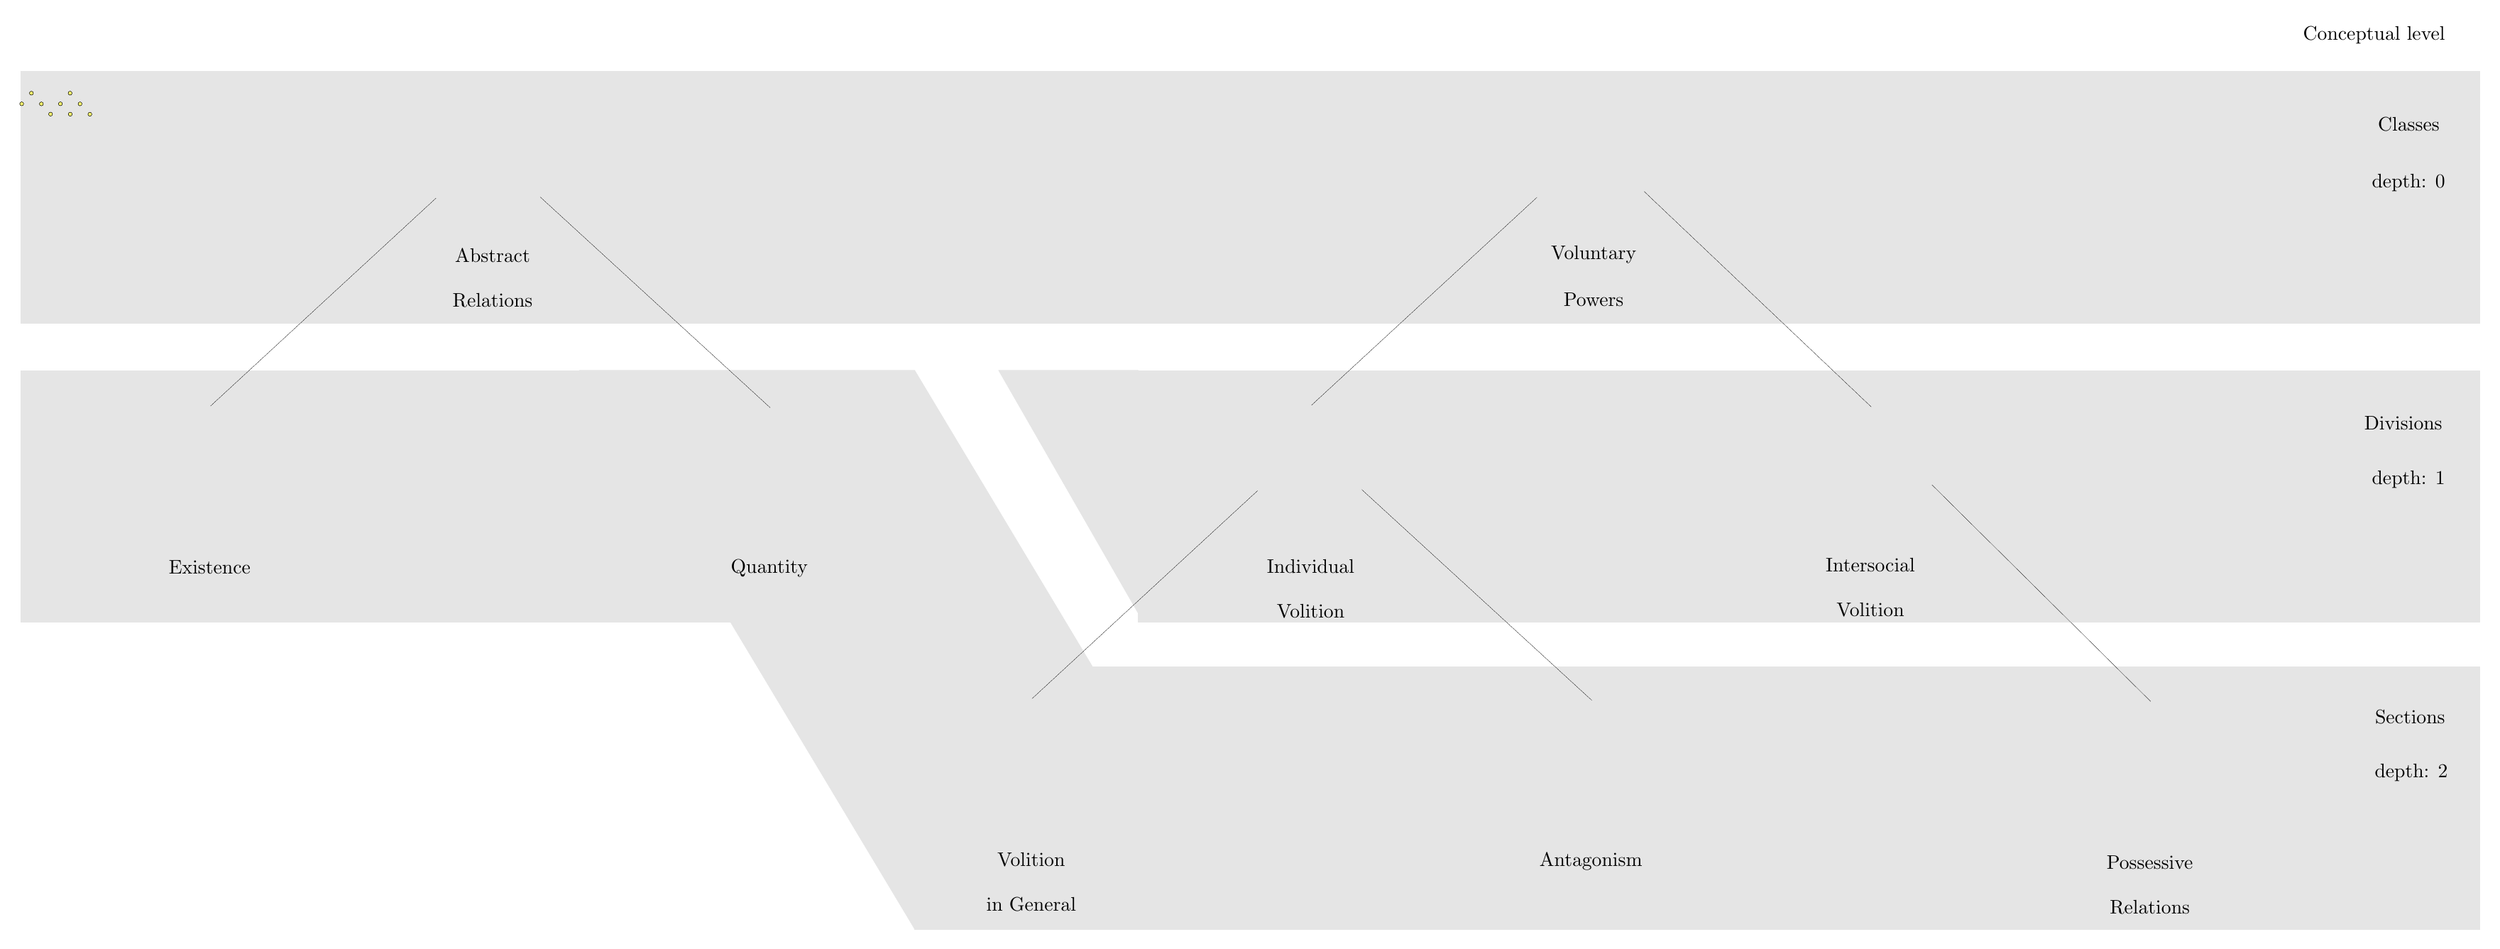
\begin{tikzpicture}
\pgftransformxscale{1.000000}
\pgftransformyscale{-1.000000}
\definecolor{dialinecolor}{rgb}{0.000000, 0.000000, 0.000000}
\pgfsetstrokecolor{dialinecolor}
\definecolor{dialinecolor}{rgb}{1.000000, 1.000000, 1.000000}
\pgfsetfillcolor{dialinecolor}
\pgfsetlinewidth{0.100000\du}
\pgfsetdash{}{0pt}
\pgfsetdash{}{0pt}
\pgfsetbuttcap
\pgfsetmiterjoin
\pgfsetlinewidth{0.100000\du}
\pgfsetbuttcap
\pgfsetmiterjoin
\pgfsetdash{}{0pt}
\definecolor{dialinecolor}{rgb}{0.898039, 0.898039, 0.898039}
\pgfsetfillcolor{dialinecolor}
\fill (20.100000\du,5.000000\du)--(17.600000\du,5.000000\du)--(20.100000\du,9.350000\du)--(22.600000\du,9.350000\du)--cycle;
\definecolor{dialinecolor}{rgb}{0.898039, 0.898039, 0.898039}
\pgfsetstrokecolor{dialinecolor}
\draw (20.100000\du,5.000000\du)--(17.600000\du,5.000000\du)--(20.100000\du,9.350000\du)--(22.600000\du,9.350000\du)--cycle;
\pgfsetbuttcap
\pgfsetmiterjoin
\pgfsetdash{}{0pt}
\definecolor{dialinecolor}{rgb}{0.898039, 0.898039, 0.898039}
\pgfsetstrokecolor{dialinecolor}
\draw (20.100000\du,5.000000\du)--(17.600000\du,5.000000\du)--(20.100000\du,9.350000\du)--(22.600000\du,9.350000\du)--cycle;
\pgfsetlinewidth{0.100000\du}
\pgfsetdash{}{0pt}
\pgfsetdash{}{0pt}
\pgfsetmiterjoin
\definecolor{dialinecolor}{rgb}{0.898039, 0.898039, 0.898039}
\pgfsetfillcolor{dialinecolor}
\fill (20.100000\du,5.000000\du)--(20.100000\du,9.500000\du)--(44.100000\du,9.500000\du)--(44.100000\du,5.000000\du)--cycle;
\definecolor{dialinecolor}{rgb}{0.898039, 0.898039, 0.898039}
\pgfsetstrokecolor{dialinecolor}
\draw (20.100000\du,5.000000\du)--(20.100000\du,9.500000\du)--(44.100000\du,9.500000\du)--(44.100000\du,5.000000\du)--cycle;
\pgfsetlinewidth{0.100000\du}
\pgfsetdash{}{0pt}
\pgfsetdash{}{0pt}
\pgfsetmiterjoin
\definecolor{dialinecolor}{rgb}{0.898039, 0.898039, 0.898039}
\pgfsetfillcolor{dialinecolor}
\fill (0.100000\du,-0.350000\du)--(0.100000\du,4.150000\du)--(44.100000\du,4.150000\du)--(44.100000\du,-0.350000\du)--cycle;
\definecolor{dialinecolor}{rgb}{0.898039, 0.898039, 0.898039}
\pgfsetstrokecolor{dialinecolor}
\draw (0.100000\du,-0.350000\du)--(0.100000\du,4.150000\du)--(44.100000\du,4.150000\du)--(44.100000\du,-0.350000\du)--cycle;
\pgfsetlinewidth{0.100000\du}
\pgfsetdash{}{0pt}
\pgfsetdash{}{0pt}
\pgfsetmiterjoin
\definecolor{dialinecolor}{rgb}{0.898039, 0.898039, 0.898039}
\pgfsetfillcolor{dialinecolor}
\fill (16.100000\du,10.300000\du)--(16.100000\du,15.000000\du)--(44.100000\du,15.000000\du)--(44.100000\du,10.300000\du)--cycle;
\definecolor{dialinecolor}{rgb}{0.898039, 0.898039, 0.898039}
\pgfsetstrokecolor{dialinecolor}
\draw (16.100000\du,10.300000\du)--(16.100000\du,15.000000\du)--(44.100000\du,15.000000\du)--(44.100000\du,10.300000\du)--cycle;
\pgfsetlinewidth{0.100000\du}
\pgfsetdash{}{0pt}
\pgfsetdash{}{0pt}
\pgfsetbuttcap
\pgfsetmiterjoin
\pgfsetlinewidth{0.100000\du}
\pgfsetbuttcap
\pgfsetmiterjoin
\pgfsetdash{}{0pt}
\definecolor{dialinecolor}{rgb}{0.898039, 0.898039, 0.898039}
\pgfsetfillcolor{dialinecolor}
\fill (16.100000\du,5.000000\du)--(10.100000\du,5.000000\du)--(16.100000\du,15.000000\du)--(22.100000\du,15.000000\du)--cycle;
\definecolor{dialinecolor}{rgb}{0.898039, 0.898039, 0.898039}
\pgfsetstrokecolor{dialinecolor}
\draw (16.100000\du,5.000000\du)--(10.100000\du,5.000000\du)--(16.100000\du,15.000000\du)--(22.100000\du,15.000000\du)--cycle;
\pgfsetbuttcap
\pgfsetmiterjoin
\pgfsetdash{}{0pt}
\definecolor{dialinecolor}{rgb}{0.898039, 0.898039, 0.898039}
\pgfsetstrokecolor{dialinecolor}
\draw (16.100000\du,5.000000\du)--(10.100000\du,5.000000\du)--(16.100000\du,15.000000\du)--(22.100000\du,15.000000\du)--cycle;
\pgfsetlinewidth{0.100000\du}
\pgfsetdash{}{0pt}
\pgfsetdash{}{0pt}
\pgfsetmiterjoin
\definecolor{dialinecolor}{rgb}{0.898039, 0.898039, 0.898039}
\pgfsetfillcolor{dialinecolor}
\fill (0.100000\du,5.000000\du)--(0.100000\du,9.500000\du)--(16.100000\du,9.500000\du)--(16.100000\du,5.000000\du)--cycle;
\definecolor{dialinecolor}{rgb}{0.898039, 0.898039, 0.898039}
\pgfsetstrokecolor{dialinecolor}
\draw (0.100000\du,5.000000\du)--(0.100000\du,9.500000\du)--(16.100000\du,9.500000\du)--(16.100000\du,5.000000\du)--cycle;
\pgfsetlinewidth{0.100000\du}
\pgfsetdash{}{0pt}
\pgfsetdash{}{0pt}
\pgfsetbuttcap
\pgfsetmiterjoin
\pgfsetlinewidth{0.100000\du}
\pgfsetbuttcap
\pgfsetmiterjoin
\pgfsetdash{}{0pt}
\definecolor{dialinecolor}{rgb}{1.000000, 0.984314, 0.435294}
\pgfsetfillcolor{dialinecolor}
\pgfpathellipse{\pgfpoint{8.440000\du}{1.200000\du}}{\pgfpoint{1.000000\du}{0\du}}{\pgfpoint{0\du}{1.000000\du}}
\pgfusepath{fill}
\definecolor{dialinecolor}{rgb}{0.000000, 0.000000, 0.000000}
\pgfsetstrokecolor{dialinecolor}
\pgfpathellipse{\pgfpoint{8.440000\du}{1.200000\du}}{\pgfpoint{1.000000\du}{0\du}}{\pgfpoint{0\du}{1.000000\du}}
\pgfusepath{stroke}
\pgfsetbuttcap
\pgfsetmiterjoin
\pgfsetdash{}{0pt}
\definecolor{dialinecolor}{rgb}{0.000000, 0.000000, 0.000000}
\pgfsetstrokecolor{dialinecolor}
\pgfpathellipse{\pgfpoint{8.440000\du}{1.200000\du}}{\pgfpoint{1.000000\du}{0\du}}{\pgfpoint{0\du}{1.000000\du}}
\pgfusepath{stroke}
% setfont left to latex
\definecolor{dialinecolor}{rgb}{0.000000, 0.000000, 0.000000}
\pgfsetstrokecolor{dialinecolor}
\node at (8.548750\du,2.945000\du){Abstract};
% setfont left to latex
\definecolor{dialinecolor}{rgb}{0.000000, 0.000000, 0.000000}
\pgfsetstrokecolor{dialinecolor}
\node at (8.548750\du,3.745000\du){Relations};
\pgfsetlinewidth{0.100000\du}
\pgfsetdash{}{0pt}
\pgfsetdash{}{0pt}
\pgfsetbuttcap
{
\definecolor{dialinecolor}{rgb}{0.000000, 0.000000, 0.000000}
\pgfsetfillcolor{dialinecolor}
% was here!!!
\definecolor{dialinecolor}{rgb}{0.000000, 0.000000, 0.000000}
\pgfsetstrokecolor{dialinecolor}
\draw (13.515100\du,5.670080\du)--(9.400000\du,1.900000\du);
}
\pgfsetlinewidth{0.100000\du}
\pgfsetdash{}{0pt}
\pgfsetdash{}{0pt}
\pgfsetbuttcap
\pgfsetmiterjoin
\pgfsetlinewidth{0.100000\du}
\pgfsetbuttcap
\pgfsetmiterjoin
\pgfsetdash{}{0pt}
\definecolor{dialinecolor}{rgb}{1.000000, 0.984314, 0.435294}
\pgfsetfillcolor{dialinecolor}
\pgfpathellipse{\pgfpoint{13.515100\du}{6.670080\du}}{\pgfpoint{1.000000\du}{0\du}}{\pgfpoint{0\du}{1.000000\du}}
\pgfusepath{fill}
\definecolor{dialinecolor}{rgb}{0.000000, 0.000000, 0.000000}
\pgfsetstrokecolor{dialinecolor}
\pgfpathellipse{\pgfpoint{13.515100\du}{6.670080\du}}{\pgfpoint{1.000000\du}{0\du}}{\pgfpoint{0\du}{1.000000\du}}
\pgfusepath{stroke}
\pgfsetbuttcap
\pgfsetmiterjoin
\pgfsetdash{}{0pt}
\definecolor{dialinecolor}{rgb}{0.000000, 0.000000, 0.000000}
\pgfsetstrokecolor{dialinecolor}
\pgfpathellipse{\pgfpoint{13.515100\du}{6.670080\du}}{\pgfpoint{1.000000\du}{0\du}}{\pgfpoint{0\du}{1.000000\du}}
\pgfusepath{stroke}
% setfont left to latex
\definecolor{dialinecolor}{rgb}{0.000000, 0.000000, 0.000000}
\pgfsetstrokecolor{dialinecolor}
\node at (13.500000\du,8.550000\du){Quantity};
\pgfsetlinewidth{0.100000\du}
\pgfsetdash{}{0pt}
\pgfsetdash{}{0pt}
\pgfsetbuttcap
{
\definecolor{dialinecolor}{rgb}{0.000000, 0.000000, 0.000000}
\pgfsetfillcolor{dialinecolor}
% was here!!!
\definecolor{dialinecolor}{rgb}{0.000000, 0.000000, 0.000000}
\pgfsetstrokecolor{dialinecolor}
\draw (7.536250\du,1.919950\du)--(3.501330\du,5.640030\du);
}
\pgfsetlinewidth{0.100000\du}
\pgfsetdash{}{0pt}
\pgfsetdash{}{0pt}
\pgfsetbuttcap
\pgfsetmiterjoin
\pgfsetlinewidth{0.100000\du}
\pgfsetbuttcap
\pgfsetmiterjoin
\pgfsetdash{}{0pt}
\definecolor{dialinecolor}{rgb}{1.000000, 0.984314, 0.435294}
\pgfsetfillcolor{dialinecolor}
\pgfpathellipse{\pgfpoint{3.501330\du}{6.640030\du}}{\pgfpoint{1.000000\du}{0\du}}{\pgfpoint{0\du}{1.000000\du}}
\pgfusepath{fill}
\definecolor{dialinecolor}{rgb}{0.000000, 0.000000, 0.000000}
\pgfsetstrokecolor{dialinecolor}
\pgfpathellipse{\pgfpoint{3.501330\du}{6.640030\du}}{\pgfpoint{1.000000\du}{0\du}}{\pgfpoint{0\du}{1.000000\du}}
\pgfusepath{stroke}
\pgfsetbuttcap
\pgfsetmiterjoin
\pgfsetdash{}{0pt}
\definecolor{dialinecolor}{rgb}{0.000000, 0.000000, 0.000000}
\pgfsetstrokecolor{dialinecolor}
\pgfpathellipse{\pgfpoint{3.501330\du}{6.640030\du}}{\pgfpoint{1.000000\du}{0\du}}{\pgfpoint{0\du}{1.000000\du}}
\pgfusepath{stroke}
% setfont left to latex
\definecolor{dialinecolor}{rgb}{0.000000, 0.000000, 0.000000}
\pgfsetstrokecolor{dialinecolor}
\node at (3.486250\du,8.519950\du){Existence};
\pgfsetlinewidth{0.100000\du}
\pgfsetdash{}{0pt}
\pgfsetdash{}{0pt}
\pgfsetbuttcap
\pgfsetmiterjoin
\pgfsetlinewidth{0.100000\du}
\pgfsetbuttcap
\pgfsetmiterjoin
\pgfsetdash{}{0pt}
\definecolor{dialinecolor}{rgb}{1.000000, 0.984314, 0.435294}
\pgfsetfillcolor{dialinecolor}
\pgfpathellipse{\pgfpoint{28.138800\du}{1.185000\du}}{\pgfpoint{1.000000\du}{0\du}}{\pgfpoint{0\du}{1.000000\du}}
\pgfusepath{fill}
\definecolor{dialinecolor}{rgb}{0.000000, 0.000000, 0.000000}
\pgfsetstrokecolor{dialinecolor}
\pgfpathellipse{\pgfpoint{28.138800\du}{1.185000\du}}{\pgfpoint{1.000000\du}{0\du}}{\pgfpoint{0\du}{1.000000\du}}
\pgfusepath{stroke}
\pgfsetbuttcap
\pgfsetmiterjoin
\pgfsetdash{}{0pt}
\definecolor{dialinecolor}{rgb}{0.000000, 0.000000, 0.000000}
\pgfsetstrokecolor{dialinecolor}
\pgfpathellipse{\pgfpoint{28.138800\du}{1.185000\du}}{\pgfpoint{1.000000\du}{0\du}}{\pgfpoint{0\du}{1.000000\du}}
\pgfusepath{stroke}
% setfont left to latex
\definecolor{dialinecolor}{rgb}{0.000000, 0.000000, 0.000000}
\pgfsetstrokecolor{dialinecolor}
\node at (28.247500\du,2.930000\du){Voluntary};
% setfont left to latex
\definecolor{dialinecolor}{rgb}{0.000000, 0.000000, 0.000000}
\pgfsetstrokecolor{dialinecolor}
\node at (28.247500\du,3.730000\du){Powers};
\pgfsetlinewidth{0.100000\du}
\pgfsetdash{}{0pt}
\pgfsetdash{}{0pt}
\pgfsetbuttcap
{
\definecolor{dialinecolor}{rgb}{0.000000, 0.000000, 0.000000}
\pgfsetfillcolor{dialinecolor}
% was here!!!
\definecolor{dialinecolor}{rgb}{0.000000, 0.000000, 0.000000}
\pgfsetstrokecolor{dialinecolor}
\draw (33.213800\du,5.655080\du)--(29.150000\du,1.800000\du);
}
\pgfsetlinewidth{0.100000\du}
\pgfsetdash{}{0pt}
\pgfsetdash{}{0pt}
\pgfsetbuttcap
\pgfsetmiterjoin
\pgfsetlinewidth{0.100000\du}
\pgfsetbuttcap
\pgfsetmiterjoin
\pgfsetdash{}{0pt}
\definecolor{dialinecolor}{rgb}{1.000000, 0.984314, 0.435294}
\pgfsetfillcolor{dialinecolor}
\pgfpathellipse{\pgfpoint{33.213800\du}{6.655080\du}}{\pgfpoint{1.000000\du}{0\du}}{\pgfpoint{0\du}{1.000000\du}}
\pgfusepath{fill}
\definecolor{dialinecolor}{rgb}{0.000000, 0.000000, 0.000000}
\pgfsetstrokecolor{dialinecolor}
\pgfpathellipse{\pgfpoint{33.213800\du}{6.655080\du}}{\pgfpoint{1.000000\du}{0\du}}{\pgfpoint{0\du}{1.000000\du}}
\pgfusepath{stroke}
\pgfsetbuttcap
\pgfsetmiterjoin
\pgfsetdash{}{0pt}
\definecolor{dialinecolor}{rgb}{0.000000, 0.000000, 0.000000}
\pgfsetstrokecolor{dialinecolor}
\pgfpathellipse{\pgfpoint{33.213800\du}{6.655080\du}}{\pgfpoint{1.000000\du}{0\du}}{\pgfpoint{0\du}{1.000000\du}}
\pgfusepath{stroke}
% setfont left to latex
\definecolor{dialinecolor}{rgb}{0.000000, 0.000000, 0.000000}
\pgfsetstrokecolor{dialinecolor}
\node at (33.198800\du,8.485000\du){Intersocial};
% setfont left to latex
\definecolor{dialinecolor}{rgb}{0.000000, 0.000000, 0.000000}
\pgfsetstrokecolor{dialinecolor}
\node at (33.198800\du,9.285000\du){Volition};
\pgfsetlinewidth{0.100000\du}
\pgfsetdash{}{0pt}
\pgfsetdash{}{0pt}
\pgfsetbuttcap
{
\definecolor{dialinecolor}{rgb}{0.000000, 0.000000, 0.000000}
\pgfsetfillcolor{dialinecolor}
% was here!!!
\definecolor{dialinecolor}{rgb}{0.000000, 0.000000, 0.000000}
\pgfsetstrokecolor{dialinecolor}
\draw (27.235000\du,1.904950\du)--(23.200100\du,5.625030\du);
}
\pgfsetlinewidth{0.100000\du}
\pgfsetdash{}{0pt}
\pgfsetdash{}{0pt}
\pgfsetbuttcap
\pgfsetmiterjoin
\pgfsetlinewidth{0.100000\du}
\pgfsetbuttcap
\pgfsetmiterjoin
\pgfsetdash{}{0pt}
\definecolor{dialinecolor}{rgb}{1.000000, 0.984314, 0.435294}
\pgfsetfillcolor{dialinecolor}
\pgfpathellipse{\pgfpoint{23.200100\du}{6.625030\du}}{\pgfpoint{1.000000\du}{0\du}}{\pgfpoint{0\du}{1.000000\du}}
\pgfusepath{fill}
\definecolor{dialinecolor}{rgb}{0.000000, 0.000000, 0.000000}
\pgfsetstrokecolor{dialinecolor}
\pgfpathellipse{\pgfpoint{23.200100\du}{6.625030\du}}{\pgfpoint{1.000000\du}{0\du}}{\pgfpoint{0\du}{1.000000\du}}
\pgfusepath{stroke}
\pgfsetbuttcap
\pgfsetmiterjoin
\pgfsetdash{}{0pt}
\definecolor{dialinecolor}{rgb}{0.000000, 0.000000, 0.000000}
\pgfsetstrokecolor{dialinecolor}
\pgfpathellipse{\pgfpoint{23.200100\du}{6.625030\du}}{\pgfpoint{1.000000\du}{0\du}}{\pgfpoint{0\du}{1.000000\du}}
\pgfusepath{stroke}
% setfont left to latex
\definecolor{dialinecolor}{rgb}{0.000000, 0.000000, 0.000000}
\pgfsetstrokecolor{dialinecolor}
\node at (23.185000\du,8.504950\du){Individual};
% setfont left to latex
\definecolor{dialinecolor}{rgb}{0.000000, 0.000000, 0.000000}
\pgfsetstrokecolor{dialinecolor}
\node at (23.185000\du,9.304950\du){Volition};
\pgfsetlinewidth{0.100000\du}
\pgfsetdash{}{0pt}
\pgfsetdash{}{0pt}
\pgfsetbuttcap
{
\definecolor{dialinecolor}{rgb}{0.000000, 0.000000, 0.000000}
\pgfsetfillcolor{dialinecolor}
% was here!!!
\definecolor{dialinecolor}{rgb}{0.000000, 0.000000, 0.000000}
\pgfsetstrokecolor{dialinecolor}
\draw (28.213800\du,10.905100\du)--(24.098800\du,7.135000\du);
}
\pgfsetlinewidth{0.100000\du}
\pgfsetdash{}{0pt}
\pgfsetdash{}{0pt}
\pgfsetbuttcap
\pgfsetmiterjoin
\pgfsetlinewidth{0.100000\du}
\pgfsetbuttcap
\pgfsetmiterjoin
\pgfsetdash{}{0pt}
\definecolor{dialinecolor}{rgb}{1.000000, 0.984314, 0.435294}
\pgfsetfillcolor{dialinecolor}
\pgfpathellipse{\pgfpoint{28.213800\du}{11.905100\du}}{\pgfpoint{1.000000\du}{0\du}}{\pgfpoint{0\du}{1.000000\du}}
\pgfusepath{fill}
\definecolor{dialinecolor}{rgb}{0.000000, 0.000000, 0.000000}
\pgfsetstrokecolor{dialinecolor}
\pgfpathellipse{\pgfpoint{28.213800\du}{11.905100\du}}{\pgfpoint{1.000000\du}{0\du}}{\pgfpoint{0\du}{1.000000\du}}
\pgfusepath{stroke}
\pgfsetbuttcap
\pgfsetmiterjoin
\pgfsetdash{}{0pt}
\definecolor{dialinecolor}{rgb}{0.000000, 0.000000, 0.000000}
\pgfsetstrokecolor{dialinecolor}
\pgfpathellipse{\pgfpoint{28.213800\du}{11.905100\du}}{\pgfpoint{1.000000\du}{0\du}}{\pgfpoint{0\du}{1.000000\du}}
\pgfusepath{stroke}
% setfont left to latex
\definecolor{dialinecolor}{rgb}{0.000000, 0.000000, 0.000000}
\pgfsetstrokecolor{dialinecolor}
\node at (28.198800\du,13.785000\du){Antagonism};
\pgfsetlinewidth{0.100000\du}
\pgfsetdash{}{0pt}
\pgfsetdash{}{0pt}
\pgfsetbuttcap
{
\definecolor{dialinecolor}{rgb}{0.000000, 0.000000, 0.000000}
\pgfsetfillcolor{dialinecolor}
% was here!!!
\definecolor{dialinecolor}{rgb}{0.000000, 0.000000, 0.000000}
\pgfsetstrokecolor{dialinecolor}
\draw (22.235000\du,7.154950\du)--(18.200100\du,10.875000\du);
}
\pgfsetlinewidth{0.100000\du}
\pgfsetdash{}{0pt}
\pgfsetdash{}{0pt}
\pgfsetbuttcap
\pgfsetmiterjoin
\pgfsetlinewidth{0.100000\du}
\pgfsetbuttcap
\pgfsetmiterjoin
\pgfsetdash{}{0pt}
\definecolor{dialinecolor}{rgb}{1.000000, 0.984314, 0.435294}
\pgfsetfillcolor{dialinecolor}
\pgfpathellipse{\pgfpoint{18.200100\du}{11.875000\du}}{\pgfpoint{1.000000\du}{0\du}}{\pgfpoint{0\du}{1.000000\du}}
\pgfusepath{fill}
\definecolor{dialinecolor}{rgb}{0.000000, 0.000000, 0.000000}
\pgfsetstrokecolor{dialinecolor}
\pgfpathellipse{\pgfpoint{18.200100\du}{11.875000\du}}{\pgfpoint{1.000000\du}{0\du}}{\pgfpoint{0\du}{1.000000\du}}
\pgfusepath{stroke}
\pgfsetbuttcap
\pgfsetmiterjoin
\pgfsetdash{}{0pt}
\definecolor{dialinecolor}{rgb}{0.000000, 0.000000, 0.000000}
\pgfsetstrokecolor{dialinecolor}
\pgfpathellipse{\pgfpoint{18.200100\du}{11.875000\du}}{\pgfpoint{1.000000\du}{0\du}}{\pgfpoint{0\du}{1.000000\du}}
\pgfusepath{stroke}
% setfont left to latex
\definecolor{dialinecolor}{rgb}{0.000000, 0.000000, 0.000000}
\pgfsetstrokecolor{dialinecolor}
\node at (18.185000\du,13.755000\du){Volition};
% setfont left to latex
\definecolor{dialinecolor}{rgb}{0.000000, 0.000000, 0.000000}
\pgfsetstrokecolor{dialinecolor}
\node at (18.185000\du,14.555000\du){in General};
\pgfsetlinewidth{0.100000\du}
\pgfsetdash{}{0pt}
\pgfsetdash{}{0pt}
\pgfsetbuttcap
{
\definecolor{dialinecolor}{rgb}{0.000000, 0.000000, 0.000000}
\pgfsetfillcolor{dialinecolor}
% was here!!!
\definecolor{dialinecolor}{rgb}{0.000000, 0.000000, 0.000000}
\pgfsetstrokecolor{dialinecolor}
\draw (38.213800\du,10.925700\du)--(34.300000\du,7.050000\du);
}
\pgfsetlinewidth{0.100000\du}
\pgfsetdash{}{0pt}
\pgfsetdash{}{0pt}
\pgfsetbuttcap
\pgfsetmiterjoin
\pgfsetlinewidth{0.100000\du}
\pgfsetbuttcap
\pgfsetmiterjoin
\pgfsetdash{}{0pt}
\definecolor{dialinecolor}{rgb}{1.000000, 0.984314, 0.435294}
\pgfsetfillcolor{dialinecolor}
\pgfpathellipse{\pgfpoint{38.213800\du}{11.925700\du}}{\pgfpoint{1.000000\du}{0\du}}{\pgfpoint{0\du}{1.000000\du}}
\pgfusepath{fill}
\definecolor{dialinecolor}{rgb}{0.000000, 0.000000, 0.000000}
\pgfsetstrokecolor{dialinecolor}
\pgfpathellipse{\pgfpoint{38.213800\du}{11.925700\du}}{\pgfpoint{1.000000\du}{0\du}}{\pgfpoint{0\du}{1.000000\du}}
\pgfusepath{stroke}
\pgfsetbuttcap
\pgfsetmiterjoin
\pgfsetdash{}{0pt}
\definecolor{dialinecolor}{rgb}{0.000000, 0.000000, 0.000000}
\pgfsetstrokecolor{dialinecolor}
\pgfpathellipse{\pgfpoint{38.213800\du}{11.925700\du}}{\pgfpoint{1.000000\du}{0\du}}{\pgfpoint{0\du}{1.000000\du}}
\pgfusepath{stroke}
% setfont left to latex
\definecolor{dialinecolor}{rgb}{0.000000, 0.000000, 0.000000}
\pgfsetstrokecolor{dialinecolor}
\node at (38.198800\du,13.805600\du){Possessive};
% setfont left to latex
\definecolor{dialinecolor}{rgb}{0.000000, 0.000000, 0.000000}
\pgfsetstrokecolor{dialinecolor}
\node at (38.198800\du,14.605600\du){Relations};
% setfont left to latex
\definecolor{dialinecolor}{rgb}{0.023529, 0.658824, 0.894118}
\pgfsetstrokecolor{dialinecolor}
\node[anchor=east] at (43.600000\du,-1.000000\du){Conceptual level};
% setfont left to latex
\definecolor{dialinecolor}{rgb}{0.023529, 0.658824, 0.894118}
\pgfsetstrokecolor{dialinecolor}
\node[anchor=east] at (43.600000\du,1.650000\du){depth: 0};
% setfont left to latex
\definecolor{dialinecolor}{rgb}{0.023529, 0.658824, 0.894118}
\pgfsetstrokecolor{dialinecolor}
\node[anchor=east] at (43.600000\du,6.950000\du){depth: 1};
% setfont left to latex
\definecolor{dialinecolor}{rgb}{0.023529, 0.658824, 0.894118}
\pgfsetstrokecolor{dialinecolor}
\node[anchor=east] at (43.650000\du,12.200000\du){depth: 2};
% setfont left to latex
\definecolor{dialinecolor}{rgb}{0.023529, 0.658824, 0.894118}
\pgfsetstrokecolor{dialinecolor}
\node[anchor=east] at (43.500000\du,0.600000\du){Classes};
% setfont left to latex
\definecolor{dialinecolor}{rgb}{0.023529, 0.658824, 0.894118}
\pgfsetstrokecolor{dialinecolor}
\node[anchor=east] at (43.550000\du,5.950000\du){Divisions};
% setfont left to latex
\definecolor{dialinecolor}{rgb}{0.023529, 0.658824, 0.894118}
\pgfsetstrokecolor{dialinecolor}
\node[anchor=east] at (43.600000\du,11.200000\du){Sections};
\end{tikzpicture}

		}
	}
	\caption[]{\label{fig:Stolk2019a:Roget-ConceptualLevel} Conceptual levels (Roget's)}
\end{figure} 

It is plain to see that the three types of category in Roget's act as a level of sorts. 
\emph{Classes}, such as "Abstract Relations" and "Voluntary Powers", convey the highest level of abstraction; \emph{sections} convey the lowest. 
Intuitively, categories of a higher level of abstraction branch out only to categories of a lower level of abstraction. 
As a consequence, we do not find categories known as \emph{sections} in Roget's Thesaurus branching out into \emph{classes} or \emph{divisions}. 

These levels mentioned do not necessarily map one-to-one with tree levels. 
In Figure \ref{fig:Stolk2019a:Roget-ConceptualLevel}, for example, both \emph{divisions} and \emph{sections} may be part of the 2nd tree level (at tree depth 1). 
Other thesauri, too, use similar notions to distinguish such conceptual levels \cite{ref-HTOED} \cite{ref-LSM}. 
In the Historical Thesaurus of the Oxford English Dictionary, the first conceptual level consists of \emph{sections}, followed by \emph{categories} and lastly \emph{subcategories}. 
Here, unlike in Roget's Thesaurus, a single category can branch out to categories from both the same conceptual level and one level beyond. 
A case in point is "Freedom/liberty". This is one of the so-called \emph{categories} and branches out to a number of other \emph{categories} (including "Independence" and "Liberation") but also to \emph{subcategories} (including "Civil liberty" and "Moral freedom").


The \emph{lemon-tree} model offers terminology to express these conceptuals levels. 
Although these levels are different from tree levels, the patterns in which thee former are captured in \emph{lemon-tree} are analogous to how tree levels are captured in XKOS:
a \textbf{ConceptualLevel} represents the level, the \textbf{conceptualDepth} property is used to indicate the depth of a level and \textbf{conceptualLevels} provides a means to list all available levels. The definitions below will be followed by snippets in which these three terms are employed.
\\

\fbox{
	\parbox{0.92\textwidth}{
		\begin{definition}
			ConceptualLevel  (Class) \\	
			A collection of concepts which are considered to be at the same conceptual depth (that is, semantically distanced from the root node). This conceptual depth may for certain thesauri coincide with the tree depth, but that is not necessarily the case for all thesauri.
			\\
			
			\quad\textbf{SubClassOf:} skos:Collection
		\end{definition}
	}
}
\\

\fbox{
	\parbox{0.92\textwidth}{
		\begin{definition}
			conceptualDepth  (DatatypeProperty) \\	
			The depth of the conceptual level that groups a number of concepts. The conceptual depth in thesaurus taxonomies can only increase in a branch, but never decrease.
			
			The first conceptual level in a thesaurus is at depth 0; the next one at depth 1, etc.
			\\
			
			\quad\textbf{Domain:} ConceptualLevel $\cup$ skos:Concept
			
			\quad\textbf{Range:} xsd:integer
		\end{definition}
	}
}

\fbox{
	\parbox{0.92\textwidth}{
		\begin{definition}
			conceptualLevels  (ObjectProperty) \\	
			Provides the list of conceptual levels for a concept scheme.
			\\
			
			\quad\textbf{Domain:} skos:ConceptScheme
			
			\quad\textbf{Range:} rdf:List
		\end{definition}
	}
}
\\

%
%
%\begin{definitionbox}[colback=white]{ConceptualLevel (Class)}
%A collection of concepts which are considered to be at the same conceptual depth (that is, semantically distanced from the root node).
%
%\medskip
%\textbf{SubClassOf:} skos:Collection
%\end{definitionbox}
%
%\begin{definitionbox}[colback=white]{conceptualDepth (Property)}
%The depth of the conceptual level that groups a number of concepts. The conceptual depth in thesaurus taxonomies can only increase in a branch, but never decrease.
%The first conceptual level in a thesaurus is at depth 0; the next one at depth 1, etc.
%\end{definitionbox}
%
%\begin{definitionbox}[colback=white]{conceptualLevels (Property)}
%Provides the list of conceptual levels for a concept scheme.
%\end{definitionbox}

\noindent
\begin{minipage}[c]{\textwidth}
	\begin{lstlisting}[
	caption={A conceptual level in lemon-tree (Roget's)},
	label={lst:Stolk2019a:ConceptualLevel-Roget}
	]
<sections> a tree:ConceptualLevel ;
	skos:prefLabel "Sections"@en ;
	tree:conceptualDepth 2 ;
	skos:member <existence> ;
	skos:member <quantity> ;
	skos:member <volition-in-general> ;
	skos:member <antagonism> ;
	skos:member <possessive-relations> .
	
<rogets> a skos:ConceptScheme ;
	skos:prefLabel "Roget's Thesaurus"@en ;
	tree:conceptualLevels ( <classes> <divisions> <sections> ) .
	\end{lstlisting}
\end{minipage}

\noindent
\begin{minipage}[c]{\textwidth}
	\begin{lstlisting}[
	caption={A conceptual level in lemon-tree (HTOED)},
	label={lst:Stolk2019a:ConceptualLevel-HTOED}
	]
<categories> a tree:ConceptualLevel ;
	skos:prefLabel "Categories"@en ;
	tree:conceptualDepth 1 ;
	skos:member <freedom-liberty> ;
	skos:member <lack-of-subjection> ;
	skos:member <permission> ;
	skos:member <authority> ;
	skos:member <communication> ;
	skos:member <society> ;
	skos:member <independence> ;
	skos:member <liberation> .
	
<htoed> a skos:ConceptScheme ;
	skos:prefLabel "Historical Thesaurus of the 
	                  Oxford English Dictionary"@en ;
	tree:conceptualLevels 
	                  ( <sections> <categories> <subcategories> ) .
	\end{lstlisting}
\end{minipage}

\noindent
The next section will discuss words and their place within the topical system.

\section{Words and senses}

A thesaurus contains lexical items that have been categorized, allowing users to go from meaning to words or phrases that express that meaning. 
Such words and senses can be represented using \emph{lemon} OntoLex terminology. 
A word or phrase is captured as an OntoLex LexicalEntry and each of its senses as a LexicalSense. 
Examples thereof are presented below.

\noindent
\begin{minipage}[c]{\textwidth}
	\begin{lstlisting}[
	caption={A lexical entry in lemon-tree},
	label={lst:Stolk2019a:LexicalEntry-HTOED}
	]
<entry-freedom> a ontolex:LexicalEntry ;
	rdfs:label "freedom"@en ;
	ontolex:canonicalForm [ 
	    a ontolex:Form ;
	    ontolex:writtenRep "freedom"@en ;
	] .
	\end{lstlisting}
\end{minipage}

\noindent
\begin{minipage}[c]{\textwidth}
	\begin{lstlisting}[
	caption={A lexical sense in lemon-tree},
	label={lst:Stolk2019a:LexicalSense-HTOED}
	]
<sense-freedom-3> a ontolex:LexicalSense ;
	ontolex:isSenseOf <entry-freedom> .
	\end{lstlisting}
\end{minipage}

For further details on the notion of LexicalEntry and LexicalSense, we refer the reader to the \emph{lemon} documentation. Advice on how to best capture other aspects of lexical items (e.g., their part of speech and other labels) is provided there, too.

\subsection{Categorization}

Topical thesauri do not categorize lexical items or word-forms but lexical senses: words or phrases in a particular sense. 
This statement may at first glance appear counter-intuitive for users of thesauri, as a number of these resources simply present head-forms of a word (or phrase) as member of their categories. 
In the Shakespeare Thesaurus \cite{ref-ShT}, for instance, category “01.02 sky” contains the following item:
\begin{quotation}
	\textbf{heaven, n.}
\end{quotation}
The head-form “heaven” in this example is similar in appearance to a headword, or lemma, found in typical dictionaries. 
This gives off the appearance that thesauri categorize lexical items. The following fictitious dictionary entry, however, demonstrates otherwise.
\begin{quotation}
	\textbf{heaven, n.} 1) abode of one or more gods 2) the sky
\end{quotation}
It is evident that the “heaven, n.” entry in the Shakespeare Thesaurus, found in the category “01.02 sky”, represents the lexical item heaven in not all of its senses listed above but in only the second sense. 

Werner Hüllen, who has thoroughly researched the topical tradition of thesauri, confirms that the entries in thesauri represent senses \cite{hullen_history_2004}. 
Further confirmation that topical thesauri categorize lexical senses can be found in the online edition of the Historical Thesaurus of the Oxford English Dictionary \cite{ref-HTOED-Online}. 
This edition takes advantage of both the topical structure of the thesaurus and the full dictionary entries of the Oxford English Dictionary. 
This rich set-up allows for a closer investigation of the relation between a thesaurus and entries in a dictionary. 
Dictionary entries in the Oxford English Dictionary have a number of senses. 
Each sense listed contains a reference to a thesaurus category. 
Conversely, the thesaurus categories in this edition list the senses they contain and provide hyperlinks not simply to dictionary entries but to specific senses \emph{within} these entries. 
As such, it is evident that this thesaurus indeed categorizes senses of lexical entries, and not lexical entries as a whole. 
In the next section, we will provide more detail on categorization and how to capture it using \emph{lemon-tree}. 

\subsection{Categorization and lexicalization}

There are two forms of categorization to be found in thesauri. In the Historical Thesaurus of the Oxford English Dictionary, words in a particular sense directly express their concept. These words are said to \emph{lexicalize} that concept. 
In Figure \ref{fig:Stolk2019a:HTE}, "freedom" and "liberty" can directly be used if one wants to express "Liberty/freedom". 
This used to be the case for "freeship" and "franchise", too, in the history of the English language. 
(As this is no longer the case, these word senses are marked with a cross in front of them.) 

Such lexicalization is not present in every thesaurus, however. 
In fact, it is more often the case than not in thesauri that it is absent. 
The sample in Figure \ref{fig:Stolk2019a:ScT-categorization} has been taken from the Scots Thesaurus \cite{ref-ScT} and illustrates this lack of lexicalization. 
% Dia export had to be mended slightly:
% - dagger symbol did not appear (replaced † with $\dagger$)
\begin{figure}[htbp]
	\framebox[\textwidth]{
		\scalebox{0.65}[0.65]{
			% Graphic for TeX using PGF
% Title: C:\Users\Sander\Documents\Dropbox\PhD\images\Content-parts (ScT-2).dia
% Creator: Dia v0.97.2
% CreationDate: Sun Apr 02 17:48:04 2017
% For: Sander
% \usepackage{tikz}
% The following commands are not supported in PSTricks at present
% We define them conditionally, so when they are implemented,
% this pgf file will use them.
\ifx\du\undefined
  \newlength{\du}
\fi
\setlength{\du}{15\unitlength}
\begin{tikzpicture}
\pgftransformxscale{1.000000}
\pgftransformyscale{-1.000000}
\definecolor{dialinecolor}{rgb}{0.000000, 0.000000, 0.000000}
\pgfsetstrokecolor{dialinecolor}
\definecolor{dialinecolor}{rgb}{1.000000, 1.000000, 1.000000}
\pgfsetfillcolor{dialinecolor}
\pgfsetlinewidth{0.100000\du}
\pgfsetdash{}{0pt}
\pgfsetdash{}{0pt}
\pgfsetmiterjoin
\definecolor{dialinecolor}{rgb}{1.000000, 1.000000, 1.000000}
\pgfsetfillcolor{dialinecolor}
\fill (18.100000\du,11.000000\du)--(18.100000\du,15.600000\du)--(32.871967\du,15.600000\du)--(32.871967\du,11.000000\du)--cycle;
\definecolor{dialinecolor}{rgb}{0.000000, 0.000000, 1.000000}
\pgfsetstrokecolor{dialinecolor}
\draw (18.100000\du,11.000000\du)--(18.100000\du,15.600000\du)--(32.871967\du,15.600000\du)--(32.871967\du,11.000000\du)--cycle;
% setfont left to latex
\definecolor{dialinecolor}{rgb}{0.000000, 0.000000, 0.000000}
\pgfsetstrokecolor{dialinecolor}
\node[anchor=west] at (19.150000\du,14.350000\du){miss};
% setfont left to latex
\definecolor{dialinecolor}{rgb}{0.000000, 0.000000, 0.000000}
\pgfsetstrokecolor{dialinecolor}
\node[anchor=west] at (19.100000\du,11.800000\du){blander};
\pgfsetlinewidth{0.100000\du}
\pgfsetdash{}{0pt}
\pgfsetdash{}{0pt}
\pgfsetmiterjoin
\pgfsetbuttcap
{
\definecolor{dialinecolor}{rgb}{0.000000, 0.000000, 1.000000}
\pgfsetfillcolor{dialinecolor}
% was here!!!
\pgfsetarrowsend{stealth}
{\pgfsetcornersarced{\pgfpoint{0.000000\du}{0.000000\du}}\definecolor{dialinecolor}{rgb}{0.000000, 0.000000, 1.000000}
\pgfsetstrokecolor{dialinecolor}
\draw (18.049928\du,13.300000\du)--(14.550000\du,13.300000\du)--(14.550000\du,9.250000\du)--(14.550000\du,9.250000\du);
}}
\definecolor{dialinecolor}{rgb}{1.000000, 1.000000, 1.000000}
\pgfsetfillcolor{dialinecolor}
\fill (12.150000\du,10.955000\du)--(12.150000\du,11.700000\du)--(12.150000\du,11.700000\du)--(12.150000\du,10.955000\du)--cycle;
% setfont left to latex
\definecolor{dialinecolor}{rgb}{0.000000, 0.000000, 0.000000}
\pgfsetstrokecolor{dialinecolor}
\node at (12.150000\du,11.550000\du){};
\pgfsetlinewidth{0.100000\du}
\pgfsetdash{}{0pt}
\pgfsetdash{}{0pt}
\pgfsetbuttcap
\pgfsetmiterjoin
\pgfsetlinewidth{0.100000\du}
\pgfsetbuttcap
\pgfsetmiterjoin
\pgfsetdash{}{0pt}
\definecolor{dialinecolor}{rgb}{1.000000, 0.984314, 0.435294}
\pgfsetfillcolor{dialinecolor}
\pgfpathellipse{\pgfpoint{10.695000\du}{4.150000\du}}{\pgfpoint{1.000000\du}{0\du}}{\pgfpoint{0\du}{1.000000\du}}
\pgfusepath{fill}
\definecolor{dialinecolor}{rgb}{0.000000, 0.000000, 0.000000}
\pgfsetstrokecolor{dialinecolor}
\pgfpathellipse{\pgfpoint{10.695000\du}{4.150000\du}}{\pgfpoint{1.000000\du}{0\du}}{\pgfpoint{0\du}{1.000000\du}}
\pgfusepath{stroke}
\pgfsetbuttcap
\pgfsetmiterjoin
\pgfsetdash{}{0pt}
\definecolor{dialinecolor}{rgb}{0.000000, 0.000000, 0.000000}
\pgfsetstrokecolor{dialinecolor}
\pgfpathellipse{\pgfpoint{10.695000\du}{4.150000\du}}{\pgfpoint{1.000000\du}{0\du}}{\pgfpoint{0\du}{1.000000\du}}
\pgfusepath{stroke}
\pgfsetlinewidth{0.100000\du}
\pgfsetdash{}{0pt}
\pgfsetdash{}{0pt}
\pgfsetbuttcap
\pgfsetmiterjoin
\pgfsetlinewidth{0.100000\du}
\pgfsetbuttcap
\pgfsetmiterjoin
\pgfsetdash{}{0pt}
\definecolor{dialinecolor}{rgb}{1.000000, 0.984314, 0.435294}
\pgfsetfillcolor{dialinecolor}
\pgfpathellipse{\pgfpoint{6.940000\du}{1.200000\du}}{\pgfpoint{1.000000\du}{0\du}}{\pgfpoint{0\du}{1.000000\du}}
\pgfusepath{fill}
\definecolor{dialinecolor}{rgb}{0.000000, 0.000000, 0.000000}
\pgfsetstrokecolor{dialinecolor}
\pgfpathellipse{\pgfpoint{6.940000\du}{1.200000\du}}{\pgfpoint{1.000000\du}{0\du}}{\pgfpoint{0\du}{1.000000\du}}
\pgfusepath{stroke}
\pgfsetbuttcap
\pgfsetmiterjoin
\pgfsetdash{}{0pt}
\definecolor{dialinecolor}{rgb}{0.000000, 0.000000, 0.000000}
\pgfsetstrokecolor{dialinecolor}
\pgfpathellipse{\pgfpoint{6.940000\du}{1.200000\du}}{\pgfpoint{1.000000\du}{0\du}}{\pgfpoint{0\du}{1.000000\du}}
\pgfusepath{stroke}
\definecolor{dialinecolor}{rgb}{1.000000, 1.000000, 1.000000}
\pgfsetfillcolor{dialinecolor}
\fill (9.663750\du,5.250000\du)--(9.663750\du,5.995000\du)--(11.726250\du,5.995000\du)--(11.726250\du,5.250000\du)--cycle;
% setfont left to latex
\definecolor{dialinecolor}{rgb}{0.000000, 0.000000, 0.000000}
\pgfsetstrokecolor{dialinecolor}
\node at (10.695000\du,5.845000\du){Crops};
\definecolor{dialinecolor}{rgb}{1.000000, 1.000000, 1.000000}
\pgfsetfillcolor{dialinecolor}
\fill (5.406250\du,2.350000\du)--(5.406250\du,3.095000\du)--(8.391250\du,3.095000\du)--(8.391250\du,2.350000\du)--cycle;
% setfont left to latex
\definecolor{dialinecolor}{rgb}{0.000000, 0.000000, 0.000000}
\pgfsetstrokecolor{dialinecolor}
\node at (6.898750\du,2.945000\du){Farming};
\pgfsetlinewidth{0.100000\du}
\pgfsetdash{}{0pt}
\pgfsetdash{}{0pt}
\pgfsetbuttcap
{
\definecolor{dialinecolor}{rgb}{0.000000, 0.000000, 0.000000}
\pgfsetfillcolor{dialinecolor}
% was here!!!
\definecolor{dialinecolor}{rgb}{0.000000, 0.000000, 0.000000}
\pgfsetstrokecolor{dialinecolor}
\draw (9.815080\du,3.320080\du)--(7.915080\du,1.870080\du);
}
\pgfsetlinewidth{0.100000\du}
\pgfsetdash{}{0pt}
\pgfsetdash{}{0pt}
\pgfsetbuttcap
\pgfsetmiterjoin
\pgfsetlinewidth{0.100000\du}
\pgfsetbuttcap
\pgfsetmiterjoin
\pgfsetdash{}{0pt}
\definecolor{dialinecolor}{rgb}{1.000000, 0.984314, 0.435294}
\pgfsetfillcolor{dialinecolor}
\pgfpathellipse{\pgfpoint{14.600000\du}{7.050000\du}}{\pgfpoint{1.000000\du}{0\du}}{\pgfpoint{0\du}{1.000000\du}}
\pgfusepath{fill}
\definecolor{dialinecolor}{rgb}{0.000000, 0.000000, 0.000000}
\pgfsetstrokecolor{dialinecolor}
\pgfpathellipse{\pgfpoint{14.600000\du}{7.050000\du}}{\pgfpoint{1.000000\du}{0\du}}{\pgfpoint{0\du}{1.000000\du}}
\pgfusepath{stroke}
\pgfsetbuttcap
\pgfsetmiterjoin
\pgfsetdash{}{0pt}
\definecolor{dialinecolor}{rgb}{0.000000, 0.000000, 0.000000}
\pgfsetstrokecolor{dialinecolor}
\pgfpathellipse{\pgfpoint{14.600000\du}{7.050000\du}}{\pgfpoint{1.000000\du}{0\du}}{\pgfpoint{0\du}{1.000000\du}}
\pgfusepath{stroke}
\definecolor{dialinecolor}{rgb}{1.000000, 1.000000, 1.000000}
\pgfsetfillcolor{dialinecolor}
\fill (13.237500\du,8.305000\du)--(13.237500\du,9.050000\du)--(15.862500\du,9.050000\du)--(15.862500\du,8.305000\du)--cycle;
% setfont left to latex
\definecolor{dialinecolor}{rgb}{0.000000, 0.000000, 0.000000}
\pgfsetstrokecolor{dialinecolor}
\node at (14.550000\du,8.900000\du){Sowing};
\pgfsetlinewidth{0.100000\du}
\pgfsetdash{}{0pt}
\pgfsetdash{}{0pt}
\pgfsetbuttcap
{
\definecolor{dialinecolor}{rgb}{0.000000, 0.000000, 0.000000}
\pgfsetfillcolor{dialinecolor}
% was here!!!
\definecolor{dialinecolor}{rgb}{0.000000, 0.000000, 0.000000}
\pgfsetstrokecolor{dialinecolor}
\draw (13.600000\du,6.400000\du)--(11.700000\du,4.950000\du);
}
% setfont left to latex
\definecolor{dialinecolor}{rgb}{0.000000, 0.000000, 0.000000}
\pgfsetstrokecolor{dialinecolor}
\node[anchor=west] at (19.095000\du,12.645000\du){happer};
% setfont left to latex
\definecolor{dialinecolor}{rgb}{0.000000, 0.000000, 0.000000}
\pgfsetstrokecolor{dialinecolor}
\node[anchor=west] at (19.095000\du,13.495000\du){heuch};
% setfont left to latex
\definecolor{dialinecolor}{rgb}{0.000000, 0.000000, 0.000000}
\pgfsetstrokecolor{dialinecolor}
\node[anchor=west] at (19.195000\du,15.095000\du){...};
% setfont left to latex
\definecolor{dialinecolor}{rgb}{0.000000, 0.000000, 0.000000}
\pgfsetstrokecolor{dialinecolor}
\node[anchor=west] at (22.036057\du,11.795000\du){(in sense 'disperse scantily')};
\pgfsetlinewidth{0.100000\du}
\pgfsetdash{}{0pt}
\pgfsetdash{}{0pt}
\pgfsetbuttcap
{
\definecolor{dialinecolor}{rgb}{0.000000, 0.000000, 0.000000}
\pgfsetfillcolor{dialinecolor}
% was here!!!
\definecolor{dialinecolor}{rgb}{0.000000, 0.000000, 0.000000}
\pgfsetstrokecolor{dialinecolor}
\draw (9.600000\du,4.850000\du)--(7.850000\du,6.150000\du);
}
\pgfsetlinewidth{0.100000\du}
\pgfsetdash{}{0pt}
\pgfsetdash{}{0pt}
\pgfsetbuttcap
\pgfsetmiterjoin
\pgfsetlinewidth{0.100000\du}
\pgfsetbuttcap
\pgfsetmiterjoin
\pgfsetdash{}{0pt}
\definecolor{dialinecolor}{rgb}{1.000000, 0.984314, 0.435294}
\pgfsetfillcolor{dialinecolor}
\pgfpathellipse{\pgfpoint{6.815080\du}{6.970080\du}}{\pgfpoint{1.000000\du}{0\du}}{\pgfpoint{0\du}{1.000000\du}}
\pgfusepath{fill}
\definecolor{dialinecolor}{rgb}{0.000000, 0.000000, 0.000000}
\pgfsetstrokecolor{dialinecolor}
\pgfpathellipse{\pgfpoint{6.815080\du}{6.970080\du}}{\pgfpoint{1.000000\du}{0\du}}{\pgfpoint{0\du}{1.000000\du}}
\pgfusepath{stroke}
\pgfsetbuttcap
\pgfsetmiterjoin
\pgfsetdash{}{0pt}
\definecolor{dialinecolor}{rgb}{0.000000, 0.000000, 0.000000}
\pgfsetstrokecolor{dialinecolor}
\pgfpathellipse{\pgfpoint{6.815080\du}{6.970080\du}}{\pgfpoint{1.000000\du}{0\du}}{\pgfpoint{0\du}{1.000000\du}}
\pgfusepath{stroke}
\definecolor{dialinecolor}{rgb}{1.000000, 1.000000, 1.000000}
\pgfsetfillcolor{dialinecolor}
\fill (4.985000\du,8.255000\du)--(4.985000\du,9.000000\du)--(8.615000\du,9.000000\du)--(8.615000\du,8.255000\du)--cycle;
% setfont left to latex
\definecolor{dialinecolor}{rgb}{0.000000, 0.000000, 0.000000}
\pgfsetstrokecolor{dialinecolor}
\node at (6.800000\du,8.850000\du){Ploughing};
\pgfsetlinewidth{0.100000\du}
\pgfsetdash{}{0pt}
\pgfsetdash{}{0pt}
\pgfsetbuttcap
{
\definecolor{dialinecolor}{rgb}{0.000000, 0.000000, 0.000000}
\pgfsetfillcolor{dialinecolor}
% was here!!!
\definecolor{dialinecolor}{rgb}{0.000000, 0.000000, 0.000000}
\pgfsetstrokecolor{dialinecolor}
\draw (5.886250\du,1.919950\du)--(4.136250\du,3.219950\du);
}
\pgfsetlinewidth{0.100000\du}
\pgfsetdash{}{0pt}
\pgfsetdash{}{0pt}
\pgfsetbuttcap
\pgfsetmiterjoin
\pgfsetlinewidth{0.100000\du}
\pgfsetbuttcap
\pgfsetmiterjoin
\pgfsetdash{}{0pt}
\definecolor{dialinecolor}{rgb}{1.000000, 0.984314, 0.435294}
\pgfsetfillcolor{dialinecolor}
\pgfpathellipse{\pgfpoint{3.101330\du}{4.040030\du}}{\pgfpoint{1.000000\du}{0\du}}{\pgfpoint{0\du}{1.000000\du}}
\pgfusepath{fill}
\definecolor{dialinecolor}{rgb}{0.000000, 0.000000, 0.000000}
\pgfsetstrokecolor{dialinecolor}
\pgfpathellipse{\pgfpoint{3.101330\du}{4.040030\du}}{\pgfpoint{1.000000\du}{0\du}}{\pgfpoint{0\du}{1.000000\du}}
\pgfusepath{stroke}
\pgfsetbuttcap
\pgfsetmiterjoin
\pgfsetdash{}{0pt}
\definecolor{dialinecolor}{rgb}{0.000000, 0.000000, 0.000000}
\pgfsetstrokecolor{dialinecolor}
\pgfpathellipse{\pgfpoint{3.101330\du}{4.040030\du}}{\pgfpoint{1.000000\du}{0\du}}{\pgfpoint{0\du}{1.000000\du}}
\pgfusepath{stroke}
\definecolor{dialinecolor}{rgb}{1.000000, 1.000000, 1.000000}
\pgfsetfillcolor{dialinecolor}
\fill (1.595000\du,5.324950\du)--(1.595000\du,6.069950\du)--(4.577500\du,6.069950\du)--(4.577500\du,5.324950\du)--cycle;
% setfont left to latex
\definecolor{dialinecolor}{rgb}{0.000000, 0.000000, 0.000000}
\pgfsetstrokecolor{dialinecolor}
\node at (3.086250\du,5.919950\du){Farmers};
% setfont left to latex
\definecolor{dialinecolor}{rgb}{0.000000, 0.000000, 0.000000}
\pgfsetstrokecolor{dialinecolor}
\node[anchor=west] at (22.041057\du,12.650000\du){(in sense 'a basket or container')};
% setfont left to latex
\definecolor{dialinecolor}{rgb}{0.000000, 0.000000, 0.000000}
\pgfsetstrokecolor{dialinecolor}
\node[anchor=west] at (22.041057\du,13.500000\du){(in sense 'earth up plants in drills')};
% setfont left to latex
\definecolor{dialinecolor}{rgb}{0.000000, 0.000000, 0.000000}
\pgfsetstrokecolor{dialinecolor}
\node[anchor=west] at (22.041057\du,14.350000\du){(in sense 'fail to germinate or grow')};
% setfont left to latex
\definecolor{dialinecolor}{rgb}{0.000000, 0.000000, 0.000000}
\pgfsetstrokecolor{dialinecolor}
\node[anchor=west] at (18.510000\du,11.845000\du){$\dagger$};
\end{tikzpicture}

		}
	}
	\caption[]{\label{fig:Stolk2019a:ScT-categorization} Sample from The Scots Thesaurus}
\end{figure}
Here, the sense ‘to disperse scantily’ of "blander" can hardly be said to directly express "Sowing". 
This is likewise the case for the sense ‘a basket or container’ of "happer". 
These senses may have a relation to the concept of "Sowing" but they do not lexicalize that concept. 
Their meaning causes them to be listed as part of the concept instead, that they are senses \emph{in} that concept, as it were.
Note that senses that lexicalize a concept are by definition senses also found \emph{in} that concept. 
In other words, lexicalization is a special form of categorization. 

For asserting that senses are lexicalizations of a concept, OntoLex offers the property \textbf{isLexicalizedSenseOf}.
For categorization, however, current vocabularies do not offer terminology expressive enough to capture the distinction with lexicalization and the connection between these two relations \cite{stolk-2017}. 
A case in point is the OntoLex property \textbf{reference}, which might appear suitable at first glance. Indeed, the property allows referring to a concept from a lexical sense. There are two problems with its use in the context of topical thesauri, however. 
Firstly, there is no mention in OntoLex of any direct relation between \textbf{isLexicalizedSenseOf} and \textbf{reference}, which leaves the important connection between lexicalization and categorization unexpressed and hinders inferring further knowledge from topical systems of thesauri. 
Secondly, the property \textbf{reference} is considered a functional one. As such, a sense may reference a single concept only using this property. However, when a sense in a thesaurus is categorized as part of a given concept, that sense is automatically also categorized as part of any parent concepts (i.e., the sense of "blander" in The Scots Thesaurus is categorized not just with "Sowing" but also with "Crops", and "Farming"). A functional characteristic therefore does not fit in this context. 
Instead, \emph{lemon-tree} offers the property \textbf{isSenseInConcept} to capture these nuances needed for topical thesauri.
\\

\fbox{
	\parbox{0.92\textwidth}{
\begin{definition}
	isSenseInConcept  (ObjectProperty) \\	
	This property relates a lexical sense to a concept that captures its meaning to some extent (that is, partially or even fully).
	\\
	
	\quad\textbf{SubPropertyOf:} dcterms:subject
	
	\quad\textbf{Domain:} ontolex:LexicalSense
	
	\quad\textbf{Range:} skos:Concept
\end{definition}
}
}
\\

The relation between \textbf{isSenseInConcept} and terminology from Ontolex has been added to the Lemon-tree model. As a result, the Ontolex property \textbf{isLexicalizedSenseOf} is asserted to be a sub property of \textbf{isSenseInConcept}. Moreover, the property \textbf{evokes} has an additional property chain of Ontolex \textbf{sense} followed by \textbf{isSenseInConcept}.
\\

\fbox{
	\parbox{0.92\textwidth}{
		\begin{definition}
			ontolex:isLexicalizedSenseOf  (ObjectProperty) \\	
			
			\quad\textbf{SubPropertyOf:} isSenseInConcept
			
			\quad\textbf{Domain:} ontolex:LexicalSense
			
			\quad\textbf{Range:} ontolex:LexicalConcept
		\end{definition}
	}
}
\\

\fbox{
	\parbox{0.92\textwidth}{
		\begin{definition}
			ontolex:evokes (ObjectProperty) \\	
			
			\quad\textbf{Domain:} ontolex:LexicalEntry
			
			\quad\textbf{Range:} ontolex:LexicalConcept
			
			\quad\textbf{PropertyChain:}  ontolex:sense o isSenseInConcept
		\end{definition}
	}
}
\\

The examples below show how both categorization and lexicalization can be captured by employing the properties \textbf{isSenseInConcept} and \textbf{isLexicalizedSenseOf}. 
Notice that the property to express lexicalization is used in the example of the Historical Thesaurus of the Oxford English Dictionary. 
There, the use of this property automatically indicates that the category is not only a SKOS \textbf{Concept}, but a concept that is expressed or lexicalized. 
Such a concept is called a \textbf{LexicalConcept} according to OntoLex. 

\noindent
\begin{minipage}[c]{\textwidth}
	\begin{lstlisting}[
	caption={Categorization in lemon-tree},
	label={lst:Stolk2019a:Categorization-ScT}
	]
<sense-happer-basket> a ontolex:LexicalSense ;
	tree:isSenseInConcept <sowing> .

<sowing> a skos:Concept .
	\end{lstlisting}
\end{minipage}

\noindent
\begin{minipage}[c]{\textwidth}
	\begin{lstlisting}[
	caption={Lexicalization in lemon-tree},
	label={lst:Stolk2019a:Lexicalization-HTOED}
	]
<sense-freedom-3> a ontolex:LexicalSense ;
	ontolex:isLexicalizedSenseOf <freedom-liberty> .

<freedom-liberty> a ontolex:LexicalConcept .
	\end{lstlisting}
\end{minipage}

It should be noted that, whenever definitions are available for senses, it is possible to make these definitions part of the topical system. 
After all, the topical system allows a user to go from meaning to items that express that meaning. 
A sense definition is just such a meaningful item. 
The snippet below shows the result of this practice when applied to The Scots Thesaurus. 
Here, an additional concept is added to the topical system. 
This concept represents the sense definition of "happer" and is lexicalized by this sense. 

\noindent
\begin{minipage}[c]{\textwidth}
	\begin{lstlisting}[
	caption={Sense definitions as concepts},
	label={lst:Stolk2019a:Sense-definitions-as-concepts}
	]
<sense-happer-basket> a ontolex:LexicalSense ;
	ontolex:isLexicalizedSenseOf <a-basket-or-container> .

<a-basket-or-container> a ontolex:LexicalConcept ;
	skos:prefLabel "a basket or container"@en 
	skos:broader <sowing> .

<sowing> a skos:Concept .
	\end{lstlisting}
\end{minipage}

This approach has a caveat: synonyms are expected to lexicalize the same concept. 
Existing thesauri may not contain information for this additional level of grouping, requiring additional efforts in their transition to a Semantic Web form.


\subsection{Synonymy}

Categories in a topical system group lexical senses into sets with a similar or related meaning. 
In some thesauri, though certainly not all, sets exist that indicate an even stronger semantic tie: one of synonymy. 
A case in point is the Historical Thesaurus of the Oxford English Dictionary, in which senses placed at the same category are deemed loosely synonymous. 
That is to say, grouped senses in this thesaurus have a similarity in meaning and are interchangeable in specific contexts. 
The introduction to the thesaurus Love, Sex, and Marriage discusses synonymy found in thesauri as follows: \cite{ref-LSM}
\begin{quotation}
\noindent
Grouping terms together in a thesaurus, even in a thesaurus as detailed as this, does not imply absolute synonymy. Many scholars doubt whether absolute interchangeability is actually possible
\end{quotation}
Instead of absolute synonymy, then, it is common to find a looser form of synonymy in thesauri. This form is referred to as near-synonymy \cite{murphy_meaning_2016}. 

Near-synonymy is evident for lexical senses that lexicalize the same concept. 
After all, such senses directly express the same meaning. 
Thus, all the senses that lexicalize category "Freedom/liberty" of the Historical Thesaurus of the Oxford English Dictionary are known to be near-synonyms. Thus, synonymy can already be captured using terminology from \emph{lemon} OntoLex. Using further vocabularies, it is also possible to link synonyms together via a direct relation between LexicalSenses, or to form groups of synonyms known as synsets if so desired \cite{ref-LEMON}. 

\noindent
\begin{minipage}[c]{\textwidth}
	\begin{lstlisting}[
	caption={Synonymy in lemon-tree},
	label={lst:Stolk2019a:Synonymy}
	]
<sense-freedom-3> a ontolex:LexicalSense ;
	ontolex:isLexicalizedSenseOf <freedom-liberty> .
<sense-freeship-2> a ontolex:LexicalSense ;
	ontolex:isLexicalizedSenseOf <freedom-liberty> .
<sense-franchise-1a> a ontolex:LexicalSense ;
	ontolex:isLexicalizedSenseOf <freedom-liberty> .
<sense-liberty1-1b> a ontolex:LexicalSense ;
	ontolex:isLexicalizedSenseOf <freedom-liberty> .
	\end{lstlisting}
\end{minipage}








\section{Conclusion}

This paper set out to analyse fundamental needs for representing topical thesauri on the Web and to supply a solution for problematic areas encountered. The standardized SKOS and \emph{lemon} vocabularies have shown to be of great value in expressing the topical system and lexical items in such a thesaurus respectively. There are, however, a few important aspects in which they fall short. The most notable two are: (1) levels that can be distinguished in a topical system and (2) a looser form of categorization than lexicalization. The novel \emph{lemon-tree} model contains terminology to fill this gap and acts as bridge between the existing Web standards. As this paper has demonstrated, \emph{lemon-tree} allows capturing a variety of topical thesauri -- each with its own particular characteristics. Indeed, the model has thus far been employed successfully in transitioning A Thesaurus of Old English \cite{ref-TOE} to linguistic linked data and has been found to be a good fit for the Mittelhochdeutsche Begriffsdatenbank \cite{ref-MHDBDB}. The full data model of \emph{lemon-tree} and its specification can be found at \url{https://w3id.org/lemon-tree#} .



%
% ---- Bibliography ----
%
\bibliographystyle{apalike}
\bibliography{Stolk2019a/library}